\documentclass[11pt,a4paper]{article}
\usepackage[T1]{fontenc}
\usepackage{lmodern}
\usepackage[utf8]{inputenc}
\usepackage[spanish,es-tabla,es-noquoting]{babel}
\usepackage[margin=1in]{geometry}
\usepackage{amsmath,amssymb,amsfonts}
\usepackage{graphicx}
\usepackage{booktabs}
\usepackage{tabularx}
\usepackage{hyperref}
\usepackage{setspace}
\usepackage{microtype}
\usepackage{subcaption}
\usepackage{placeins}

\setstretch{1.12}
\setlength{\parskip}{0.45em}
\setlength{\parindent}{0pt}
\graphicspath{{./}}

\begin{document}

\noindent
\begin{tabular*}{\textwidth}{@{}l@{\extracolsep{\fill}}r@{}}
    \begin{minipage}{0.25\textwidth}
        \IfFileExists{logo.png}{
\includegraphics[width=\linewidth, height=18mm, keepaspectratio]{logo.png}}{\textbf{UTEC}}
    \end{minipage}
    &
    \begin{minipage}{0.72\textwidth}
    \begin{flushright}
         \textbf{DS5345 · Aprendizaje por Refuerzo (2026-II)} \\
         \textbf{Informe Técnico del Proyecto} \\
         \small Docente: Percy W. Lovon Ramos
    \end{flushright}
    \end{minipage}
\end{tabular*}

\vspace{-0.15cm}
\noindent\rule{\textwidth}{0.8pt}

\vspace{0.25cm}
\begin{center}
    {\Large \textbf{Baseline Tabular para Habilidades de Fútbol en RoboCup 2D}} \\[0.15cm]
    {\large Fase 1 (P1): catálogo de tareas acotadas} \\[0.25cm]
    \textbf{Grupo BlueLock} \\[0.08cm]
    Hans Mendoza \textperiodcentered Luis Jáuregui \\[0.12cm]
    {\small \url{https://github.com/Alaprexian/Robocup_RL2026-2}}
\end{center}

\vspace{0.1cm}
\noindent\rule{\textwidth}{0.4pt}

\begin{abstract}
En lugar de abordar directamente un partido 11\,vs\,11, el enunciado propone comenzar por habilidades individuales.
Modelamos las cuatro tareas del catálogo---persecución, drible, tiro y pase~2v1---como MDPs tabulares sobre un proxy cinemático, con discretización polar alineada al radio kickable de \texttt{rcssserver}, y comparamos Monte~Carlo Control y Q-Learning bajo $\varepsilon$ fijo frente a $\varepsilon$ decreciente (3500 episodios por configuración).
Tras ajustar el tiro (alineación multi-paso) y el pase (recompensa anclada a posesión), las cuatro tareas alcanzan los criterios de éxito del enunciado en su mejor configuración.
\end{abstract}

\section{Por qué este problema y cómo lo atacamos}
RoboCup~2D es un POMDP ruidoso y competitivo: aprender ``jugar fútbol'' de cero con métodos tabulares hace explotar el espacio.
El curso propone aislar subtareas controlables, visualizar qué aprende el agente y recién después escalar a Deep~RL.

Trabajamos en Python dentro del stack Docker del starter kit, con entornos en \texttt{src/envs/} que imitan dash, giro, kick y pase sin pagar el costo de \texttt{rcssserver} en cada update de $Q$.
El proxy no reemplaza al servidor oficial (sigue siendo el destino de despliegue), pero permite experimentos reproducibles (semilla~42) y comparación justa entre algoritmos.
Los agentes (\texttt{src/agents/}) son agnósticos al tamaño de $\mathcal{A}$: leen \texttt{env.n\_actions} y guardan $Q$ indexada por estados hashables.

\section{Discretización y formalización de las tareas}
En todas usamos $\gamma=0.99$ y políticas $\varepsilon$-greedy.

\subsection{Discretización polar}
Para que $Q(s,a)$ sea tabular, convertimos observaciones continuas (distancia y ángulo relativo) en \emph{bins}.
El esquema compartido vive en \texttt{src/discretizer.py} y replica convenciones de RoboCup~2D:

\begin{table}[htbp]
\centering
\small
\begin{tabular}{@{}clp{7.2cm}@{}}
\toprule
Bin & Rango / significado & Motivación \\
\midrule
Dist.\ 0 & $d<0.8$\,m & Radio \textbf{kickable} de \texttt{rcssserver} \\
Dist.\ 1 & $[0.8,3)$\,m & Reacción cercana \\
Dist.\ 2 & $[3,8)$\,m & Media \\
Dist.\ 3 & $d\ge 8$\,m & Lejana \\
\midrule
Áng.\ 0 & $|\theta|\le 15^\circ$ & Cono frontal de dash efectivo \\
Áng.\ 1--2 & hasta $\pm 60^\circ$ & Giro parcial \\
Áng.\ 3--4 & posterior & Giro completo \\
\bottomrule
\end{tabular}
\caption{Bins polares compartidos. En persecución pura: $|\mathcal{S}|=4\times 5=20$. Las demás tareas extienden el estado con bins adicionales (meta, portero, compañero, posesión).}
\end{table}

Las tuplas de estado discretas que indexan $Q(s,a)$ en cada tarea son:

\begin{table}[htbp]
\centering
\small
\begin{tabular}{@{}llp{6.4cm}@{}}
\toprule
Tarea & Tupla $s$ & Componentes \\
\midrule
Pursuit & $(d_b,\,a_b)$ & Dist.\ y ángulo al balón (bins polares) \\
Dribbling & $(d_b,\,a_b,\,d_g,\,a_g)$ & Balón + meta rival (bins) \\
Shooting & $(d_g,\,b,\,g_k,\,f)$ & Dist.\ arco, sector corporal, bin GK, \texttt{facing\_ok} \\
Passing & $(d_c,\,a_c,\,d_d,\,a_d,\,h)$ & Compañero, defensor, posesión $h\in\{0,1\}$ \\
\bottomrule
\end{tabular}
\caption{Estado tabular por tarea (todos los campos son enteros de bins, salvo $h$ binario).}
\end{table}

\subsection{Persecución e intercepción}
El agente nace con $d_b\in[5,40]$\,m (enunciado) y orientación aleatoria.
Estado $s=(d_b,\,a_b)$ con $|\mathcal{S}|=20$; acciones: DASH fuerte/suave ($+1.2$\,/\,$+0.6$\,m) o giro $\pm 35^\circ$; horizonte $T_{\max}=120$.
La recompensa por paso combina costo temporal y \emph{término de acercamiento}:
\[
R_t = -1 + 5\bigl(d_{t-1}-d_t\bigr),
\]
con terminal $+100$ si $d_b<0.8$\,m y $-20$ por timeout.
Así se empuja a capturas cortas y se da señal densa cuando aún no hay gol de captura.

\subsection{Drible}
Estado $s=(d_b,\,a_b,\,d_g,\,a_g)$: relación al balón y a la meta rival, ambos discretizados.
Acciones: micro-pateo, carrera y giros.
Éxito: avance neto $\ge 30$\,m con posesión vigente; fallo si sale de cancha o pierde el balón varios pasos.
Implementación: en dash cerca del balón, el proxy ``pega'' la pelota delante del jugador ($\approx 0.55$\,m), aproximando posesión sin física completa de rebote.

\subsection{Tiro a puerta}
Estado $s=(d_g,\,b,\,g_k,\,f)$: distancia al arco, sector del cuerpo, bin del portero (0\,=\,abierto) y $f=\texttt{facing\_ok}$ ($|a_g|\le 20^\circ$).
Acciones: giros (no terminan el episodio) y cinco sectores de disparo; horizonte corto ($T_{\max}=8$).
Los postes usan la escala RoboCup~2D ($\pm 7.01$\,m).
Entrenamiento mixto 50/50 con/sin arquero; evaluación greedy separada (umbrales $>75\%$ abierto, $>50\%$ con portero).
El ruido del tiro crece si el cuerpo está mal alineado: de ahí la necesidad de alinear antes de patear.

\subsection{Pase y posesión 2v1}
Atacante + compañero vs defensor \emph{estocástico} (persigue el balón con velocidad aleatoria).
Estado $s=(d_c,\,a_c,\,d_d,\,a_d,\,h)$: distancia/ángulo al compañero y al defensor (bins polares) y $h=1$ si el atacante controla el balón.
Macros: pase, drible, giro y \texttt{ALEJARSE}.
Éxito conjunto: posesión $\ge 50$ pasos \emph{y} $\ge 3$ pases.
Detalles: pase moderado (no $+30$), posesión densa ($+1.2$/paso) y \texttt{ALEJARSE}.
El stun post-pase es opcional (parámetro \texttt{defender\_stun\_on\_pass}; por defecto $0$ tras ablación).

\section{Qué entrenamos}
Cuatro configuraciones por tarea:
\begin{itemize}
    \item Monte~Carlo Control On-Policy (First-Visit) con $\varepsilon=0.1$ fijo
          y con $\varepsilon_k=\max(0.05,\,1.0\cdot 0.998^{k})$.
    \item Q-Learning ($\alpha=0.1$) con los mismos esquemas de exploración.
\end{itemize}
\texttt{run\_all\_tasks.py} exporta curvas, trays y métricas.
\texttt{generate\_tray\_sets.py} produce variantes exitosas con distintas semillas
(para no depender de un único episodio ``afortunado'').

\section{Resultados: panorama}
\begin{table}[htbp]
\centering
\small
\begin{tabular}{@{}llp{5.2cm}@{}}
\toprule
Tarea & Mejor corrida & Qué observamos \\
\midrule
Pursuit & QL + $\varepsilon$ decay ($100\%$) & $\approx 31$ pasos \\
Dribbling & QL + $\varepsilon$ decay ($100\%$) & Umbral 30\,m \\
Shooting & MC + $\varepsilon$ fijo & Open $98\%$ / GK $83\%$ \\
Passing & MC + $\varepsilon$ fijo ($93\%$) & Pos.\ $\approx 51$, stun$=0$ \\
\bottomrule
\end{tabular}
\caption{Mejor configuración por tarea (últimos 100 episodios; tiro con eval greedy separada).}
\end{table}

Tiro y pase fueron los que más dependieron de alinear $R$ (y la dinámica) al criterio del enunciado, no solo de subir $G_0$.

\FloatBarrier
\section{Zoom en persecución}
\begin{table}[htbp]
\centering
\begin{tabular}{lccc}
\toprule
Configuración & Retorno $G_0$ & Pasos & Éxito \\
\midrule
MC + $\varepsilon$ decay & $148.8$ & $38.4$ & $95\%$ \\
MC + $\varepsilon$ fijo $0.1$ & $21.0$ & $80.0$ & $53\%$ \\
QL + $\varepsilon$ decay & $166.1$ & $31.4$ & $100\%$ \\
QL + $\varepsilon$ fijo $0.1$ & $157.7$ & $41.1$ & $100\%$ \\
\bottomrule
\end{tabular}
\caption{Pursuit con $d_b\in[5,40]$\,m (últimos 100 episodios).}
\end{table}

Con distancias iniciales largas, MC + $\varepsilon$ fijo queda corto: first-visit promedia retornos muy distintos (timeout vs captura) y, si la exploración no se apaga, ``ensucia'' pares $(s,a)$.
Q-Learning, al bootstrappear, es más robusto aquí.

\begin{figure}[htbp]
    \centering
    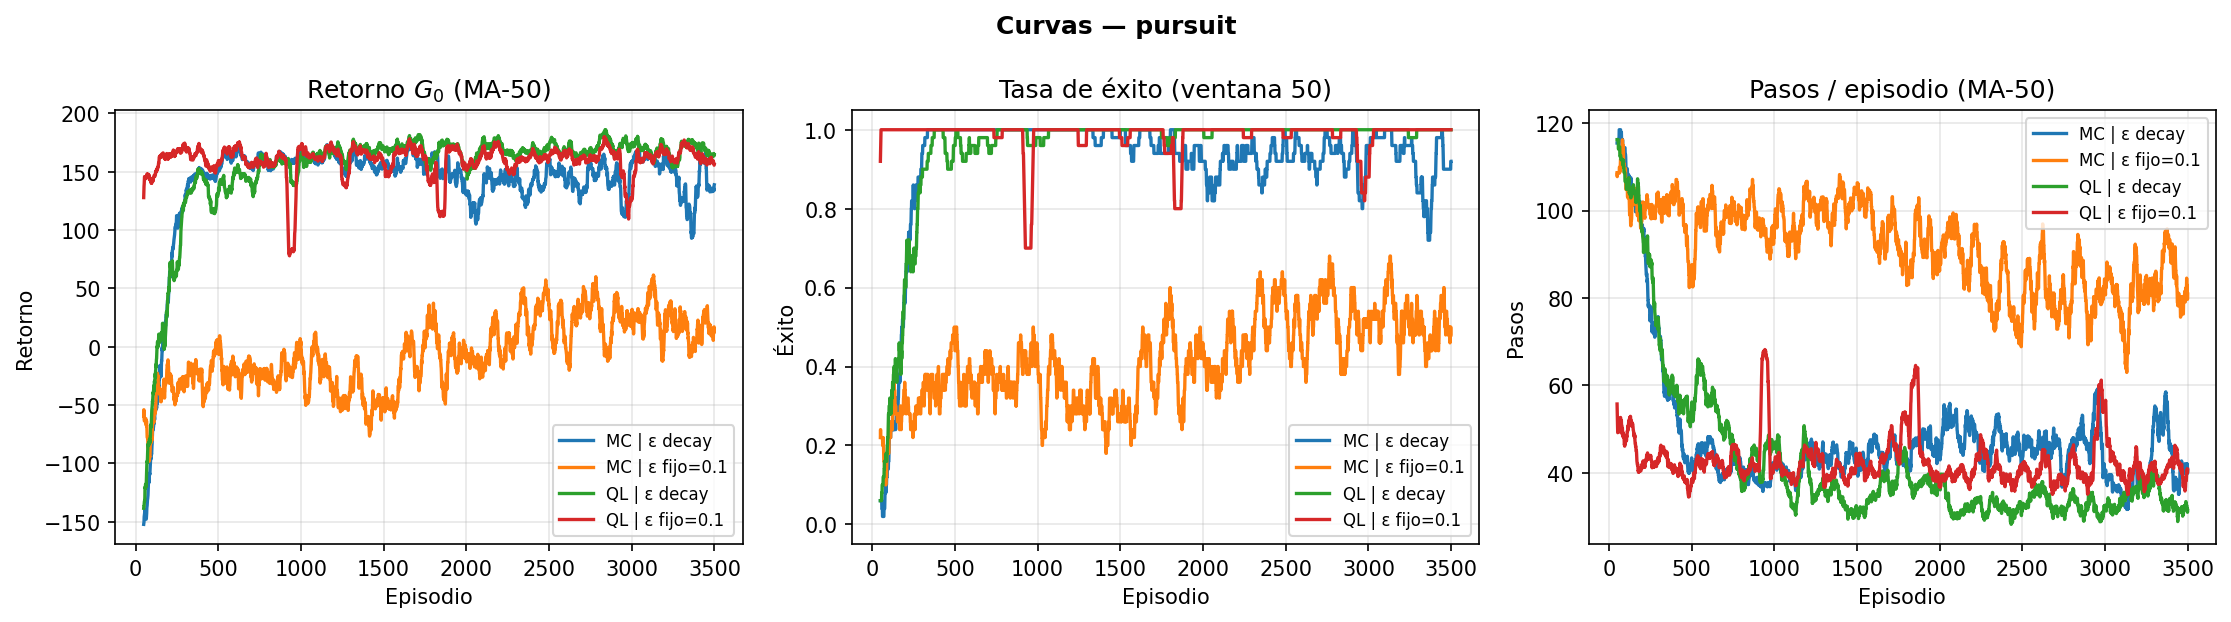
\includegraphics[width=\textwidth]{fig_pursuit_curvas.png}
    \caption{Pursuit---aprendizaje: $G_0$, tasa de éxito y pasos (MA-50).}
    \label{fig:pursuit-curvas}
\end{figure}

\begin{figure}[htbp]
    \centering
    \begin{subfigure}[t]{0.52\textwidth}
        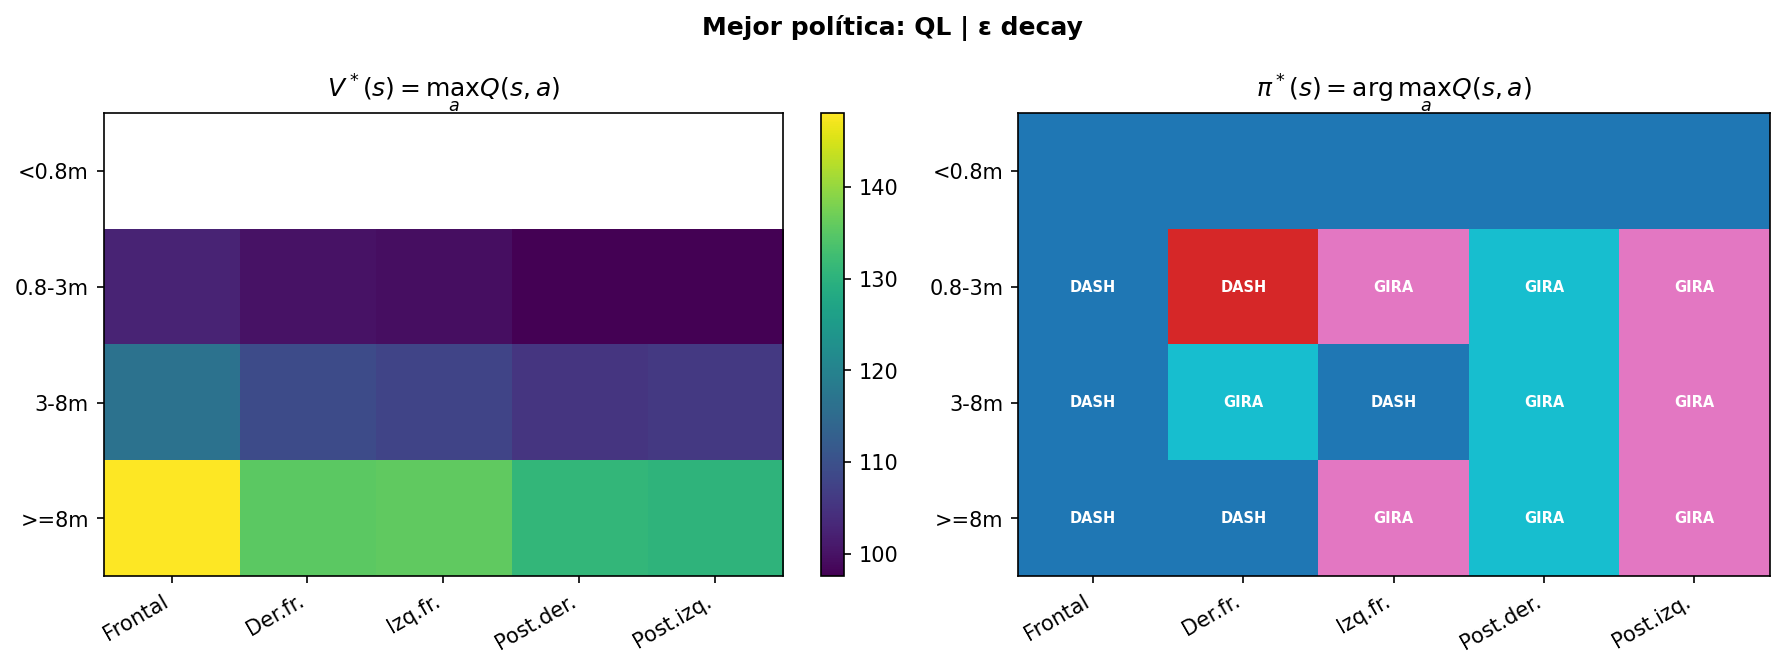
\includegraphics[width=\linewidth]{fig_pursuit_politica.png}
        \caption{$V^*$ y $\pi^*$ (mejor config.)}
        \label{fig:pursuit-pi}
    \end{subfigure}\hfill
    \begin{subfigure}[t]{0.46\textwidth}
        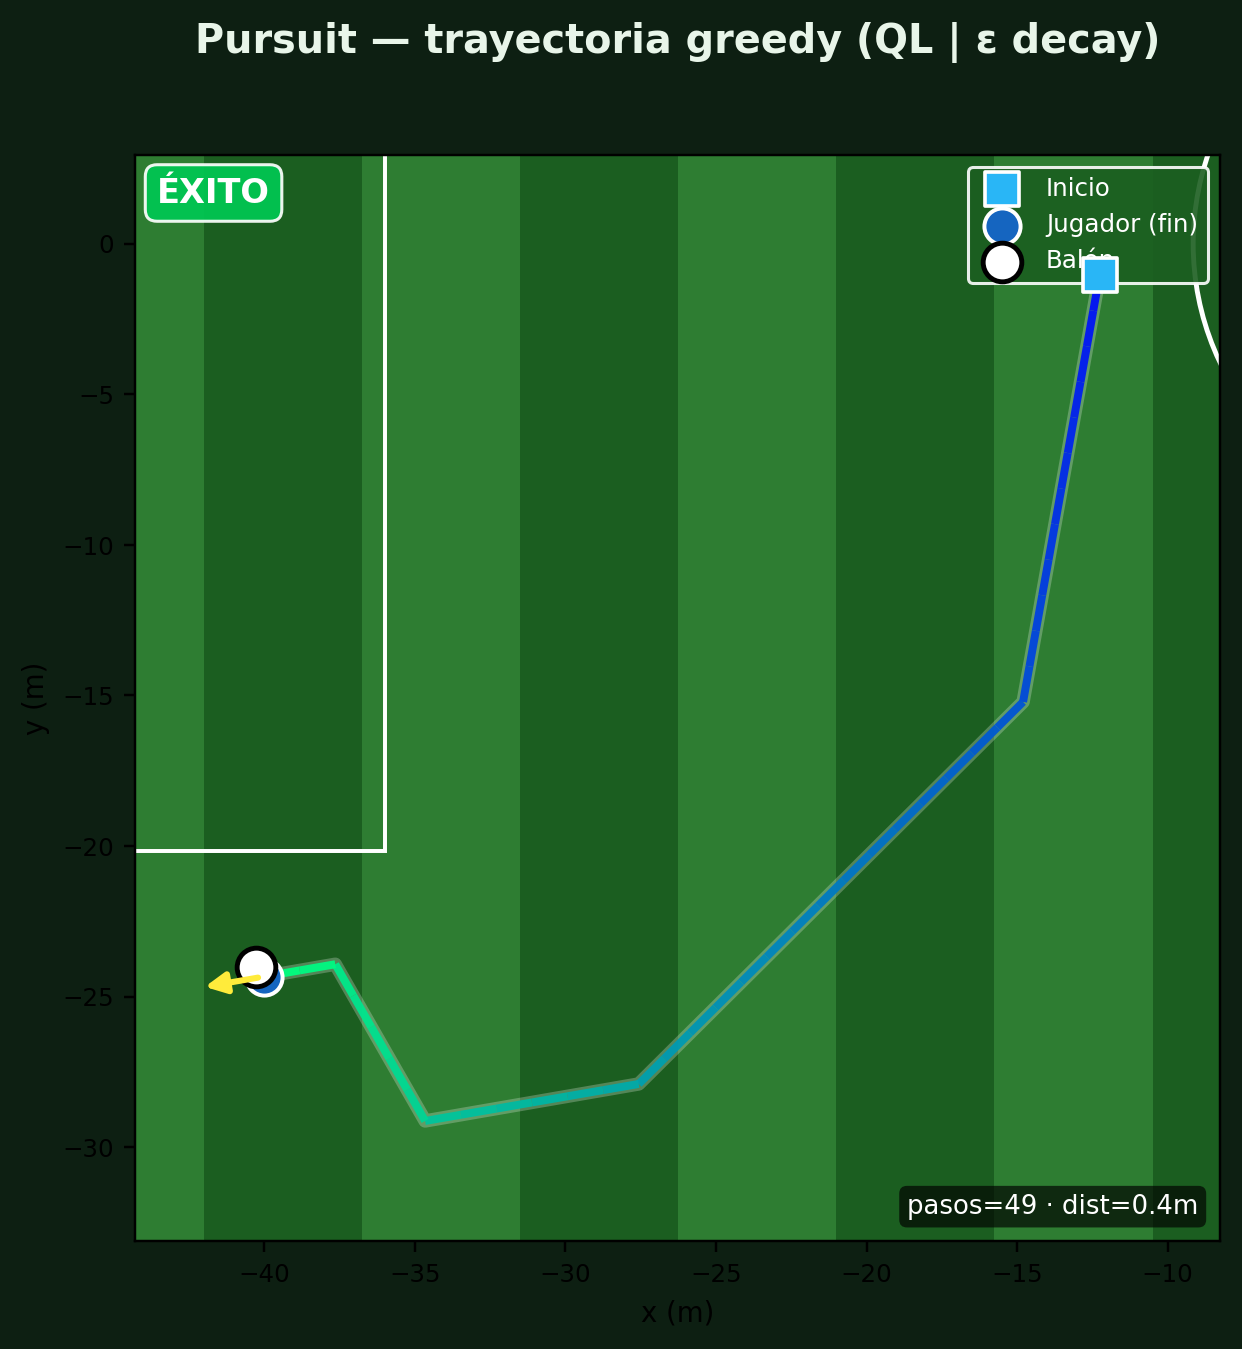
\includegraphics[width=\linewidth]{fig_pursuit_tray.png}
        \caption{Trayectoria greedy canónica}
        \label{fig:pursuit-tray}
    \end{subfigure}
    \caption{Pursuit---política tabular y un episodio greedy típico (``alinear y empujar'').}
    \label{fig:pursuit-viz}
\end{figure}

\FloatBarrier
\section{Drible}
El shaping (acercarse a la meta + castigo por perder posesión) basta para una política estable; dash con balón cerca rinde más que patadas fuertes.

\begin{figure}[htbp]
    \centering
    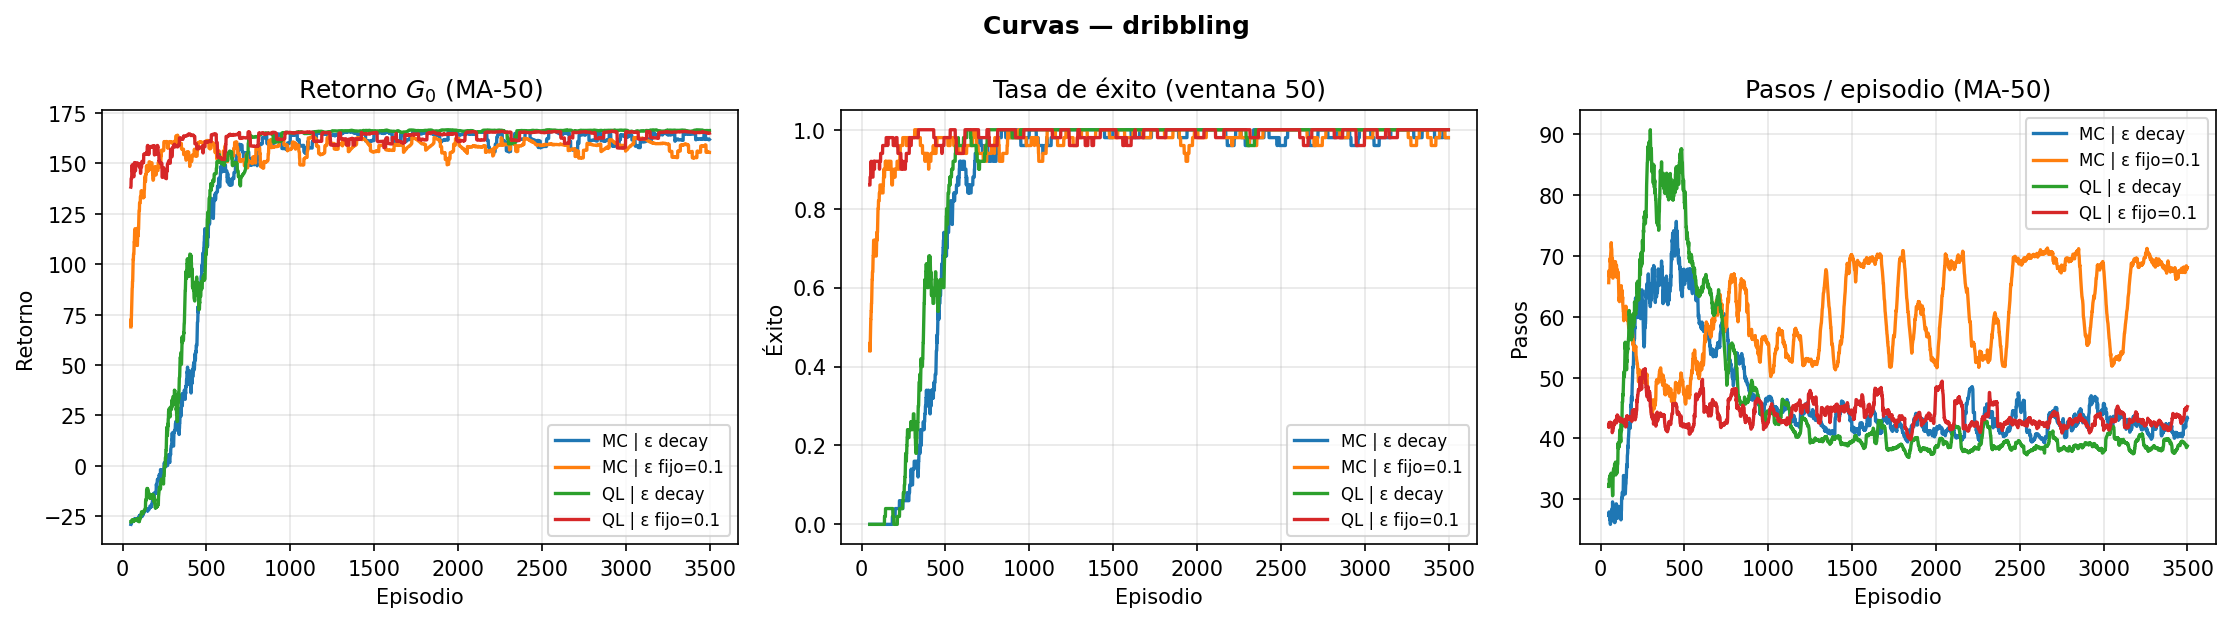
\includegraphics[width=\textwidth]{fig_dribbling_curvas.png}
    \caption{Drible---aprendizaje: las cuatro configs terminan altas; QL+$\varepsilon$ decay es la más ágil ($\approx 39$ pasos, $100\%$).}
    \label{fig:drib-curvas}
\end{figure}

\begin{figure}[htbp]
    \centering
    \begin{subfigure}[t]{0.38\textwidth}
        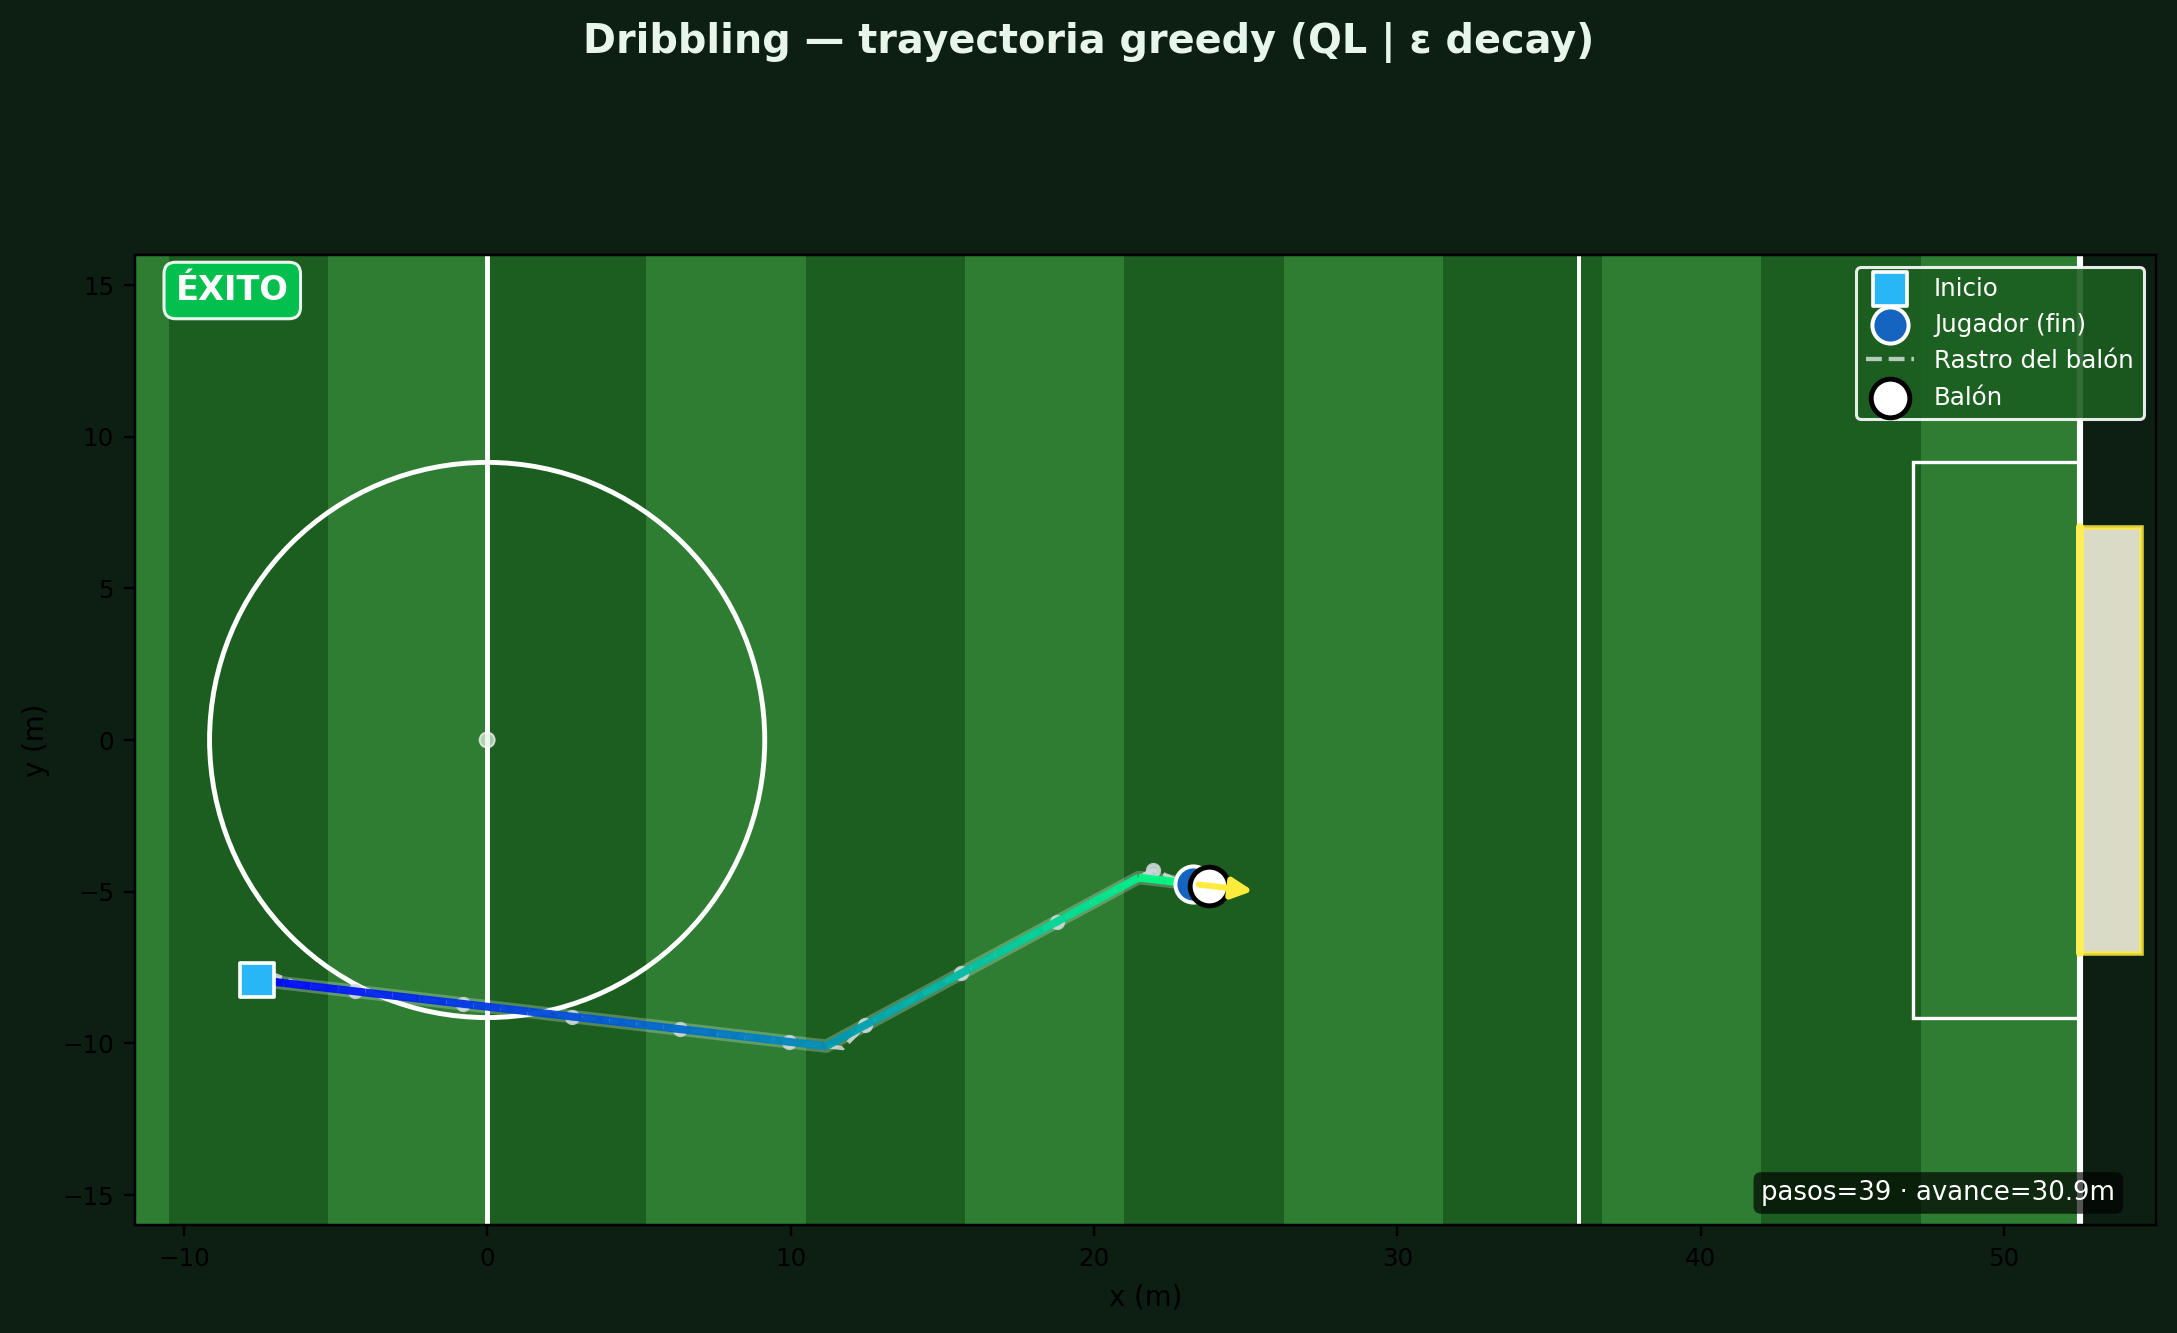
\includegraphics[width=\linewidth]{fig_dribbling_tray.png}
        \caption*{Canónica}
    \end{subfigure}\hfill
    \begin{subfigure}[t]{0.28\textwidth}
        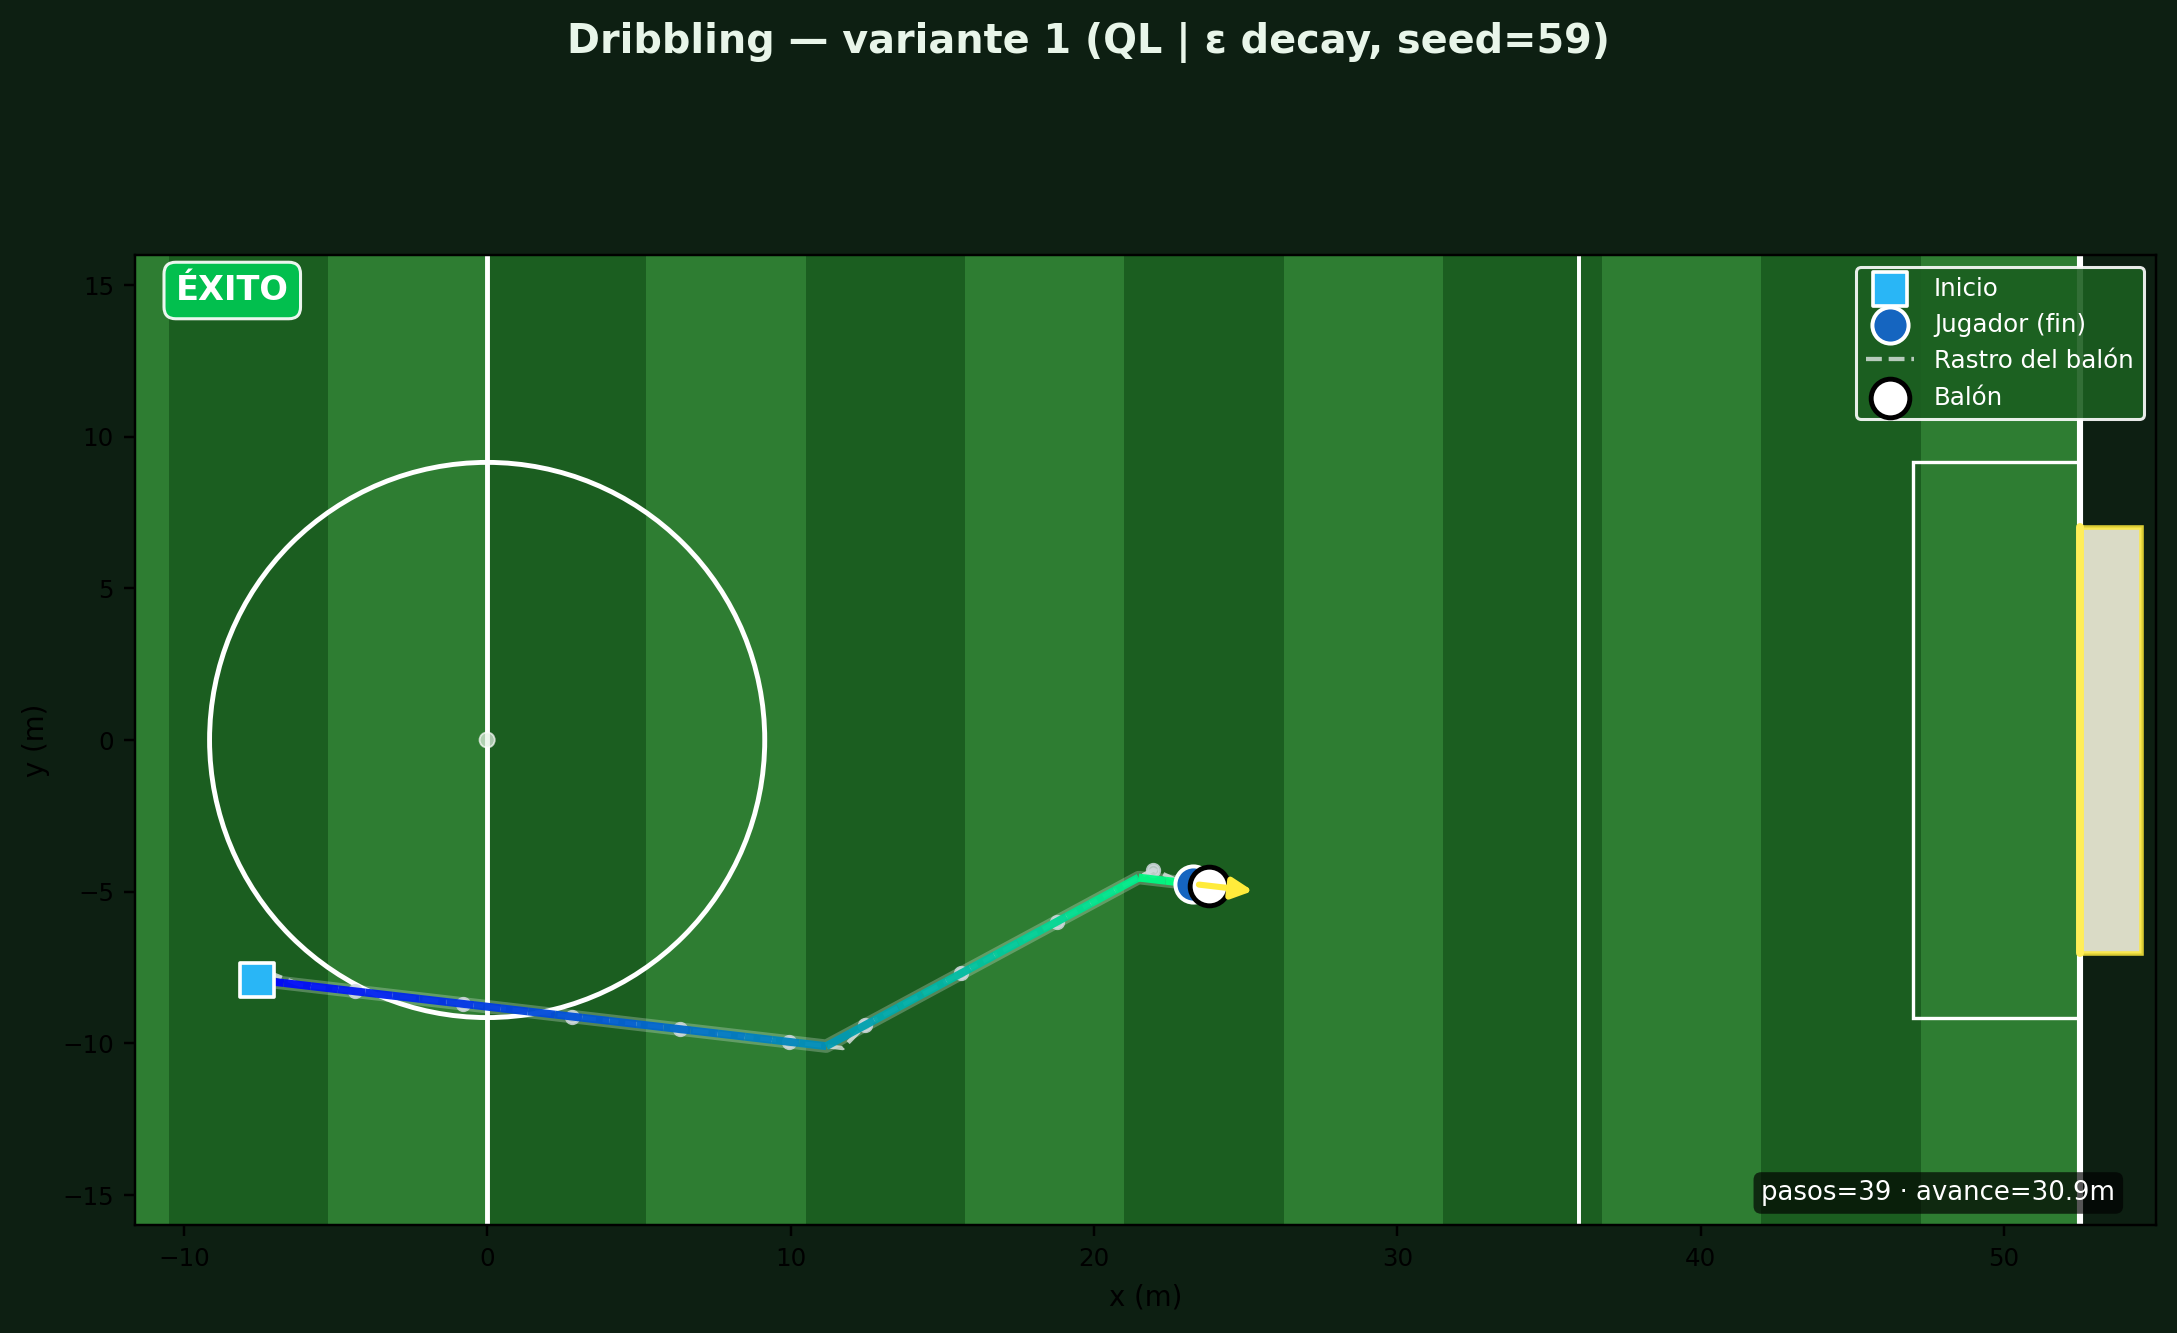
\includegraphics[width=\linewidth]{set_dribbling_01.png}
        \caption*{Seed 59}
    \end{subfigure}\hfill
    \begin{subfigure}[t]{0.28\textwidth}
        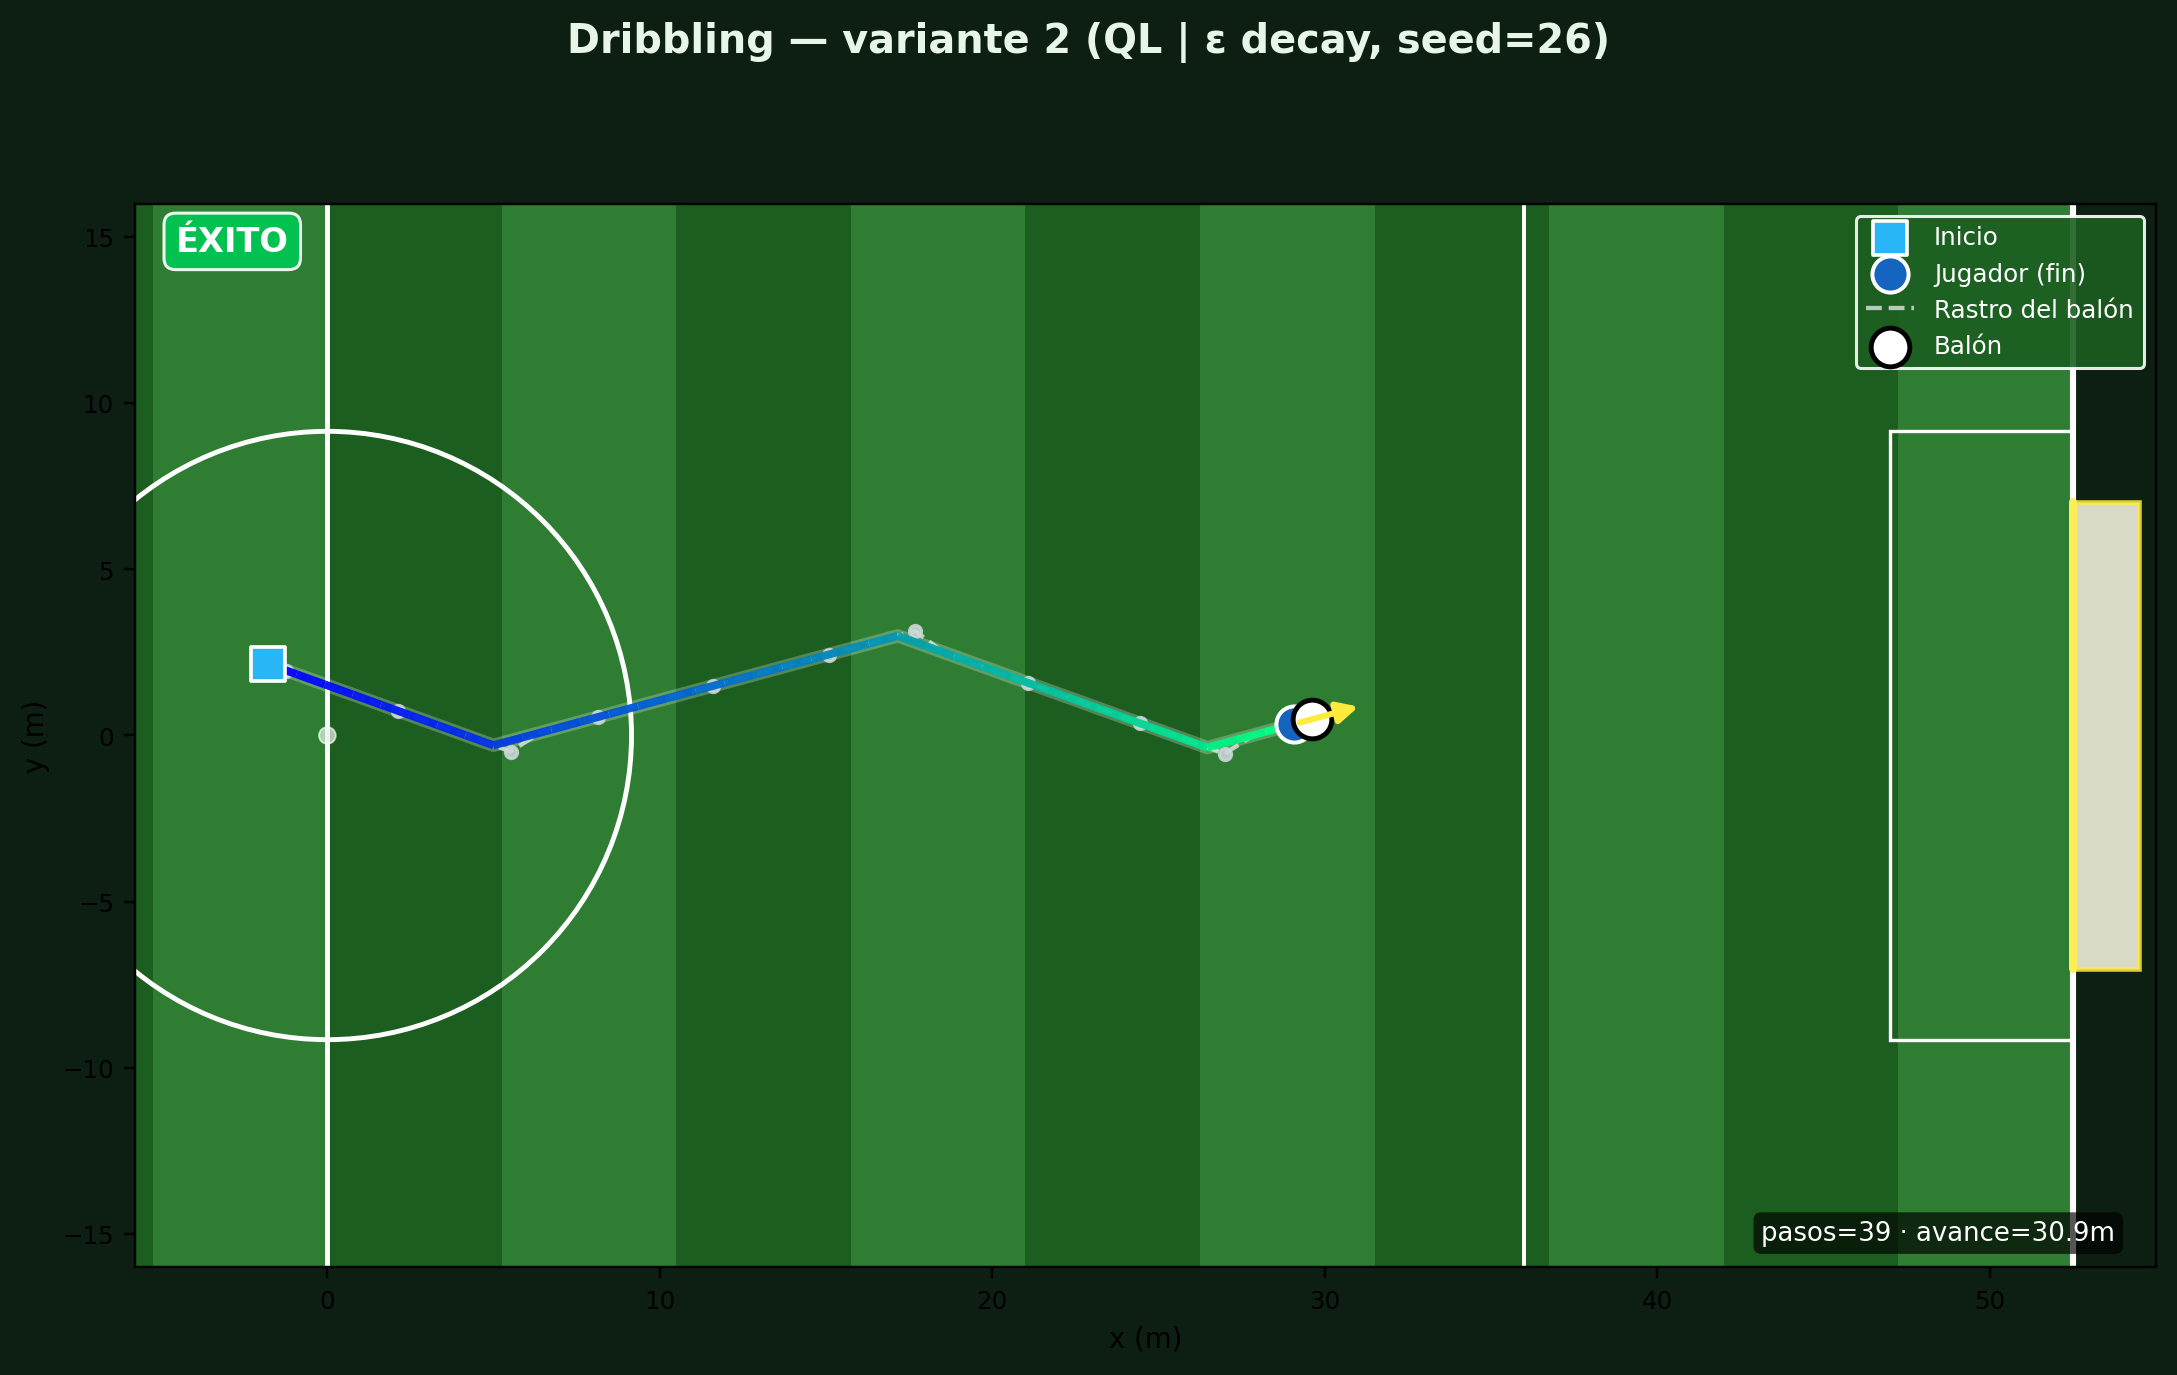
\includegraphics[width=\linewidth]{set_dribbling_02.png}
        \caption*{Seed 26}
    \end{subfigure}
    \caption{Drible---trayectorias greedy (avance $>30$\,m con posesión).}
    \label{fig:drib-viz}
\end{figure}

\FloatBarrier
\section{Tiro}
El cambio clave fue permitir alineación antes del disparo.
MC + $\varepsilon$ fijo alcanza $98\%$ abierto y $83\%$ con portero en eval greedy (umbrales $75\%/50\%$).

\begin{figure}[htbp]
    \centering
    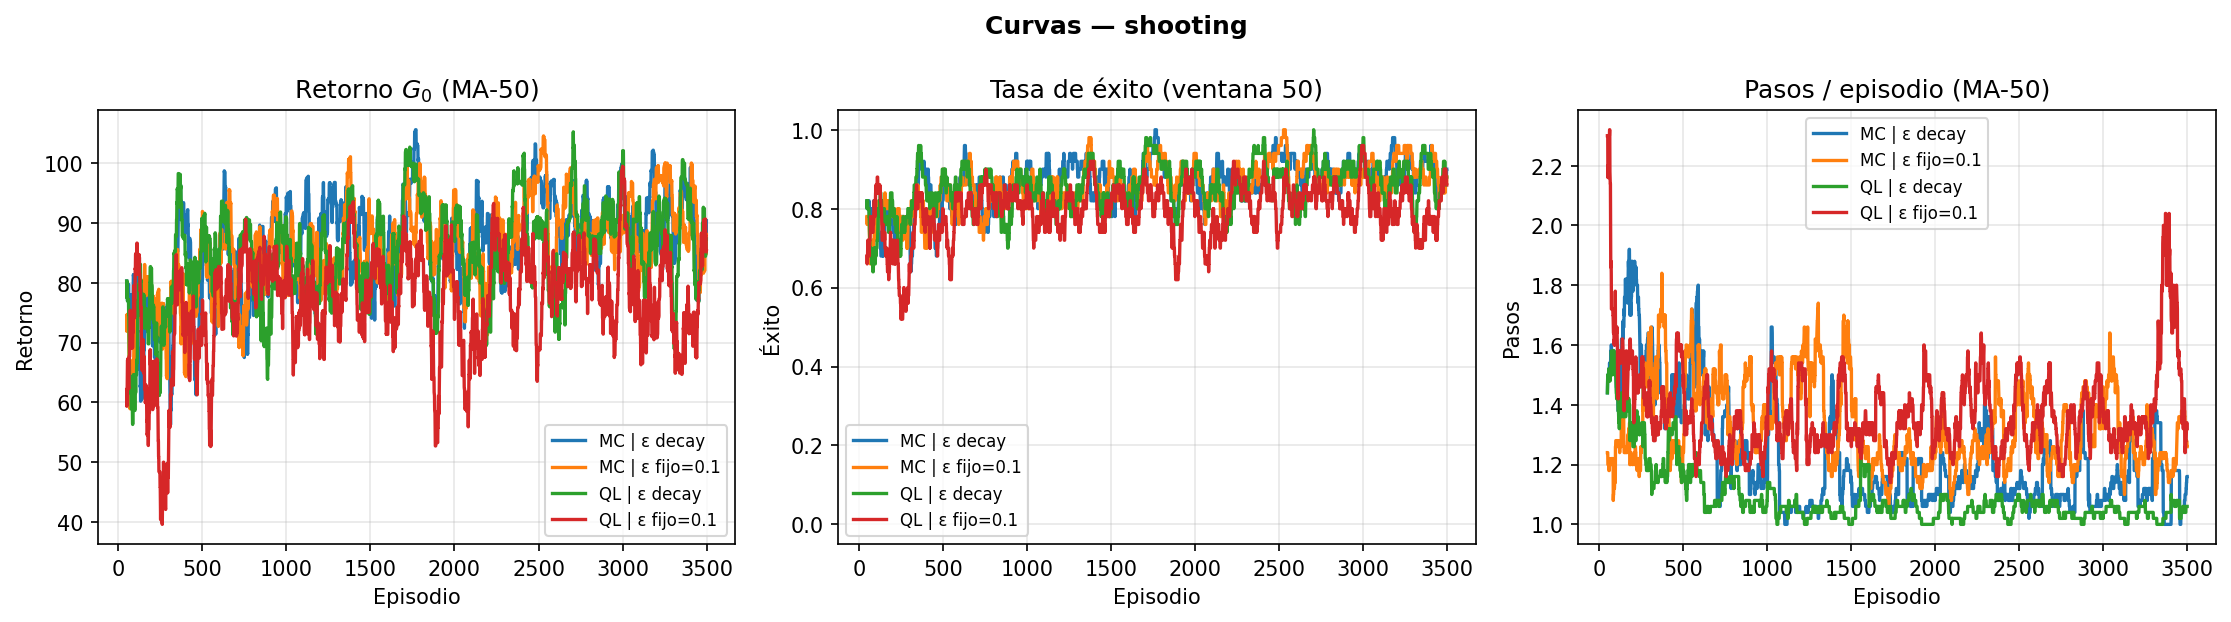
\includegraphics[width=\textwidth]{fig_shooting_curvas.png}
    \caption{Tiro---aprendizaje bajo mixto open/GK (episodios cortos: alinear y patear).}
    \label{fig:shot-curvas}
\end{figure}

\begin{figure}[htbp]
    \centering
    \begin{subfigure}[t]{0.48\textwidth}
        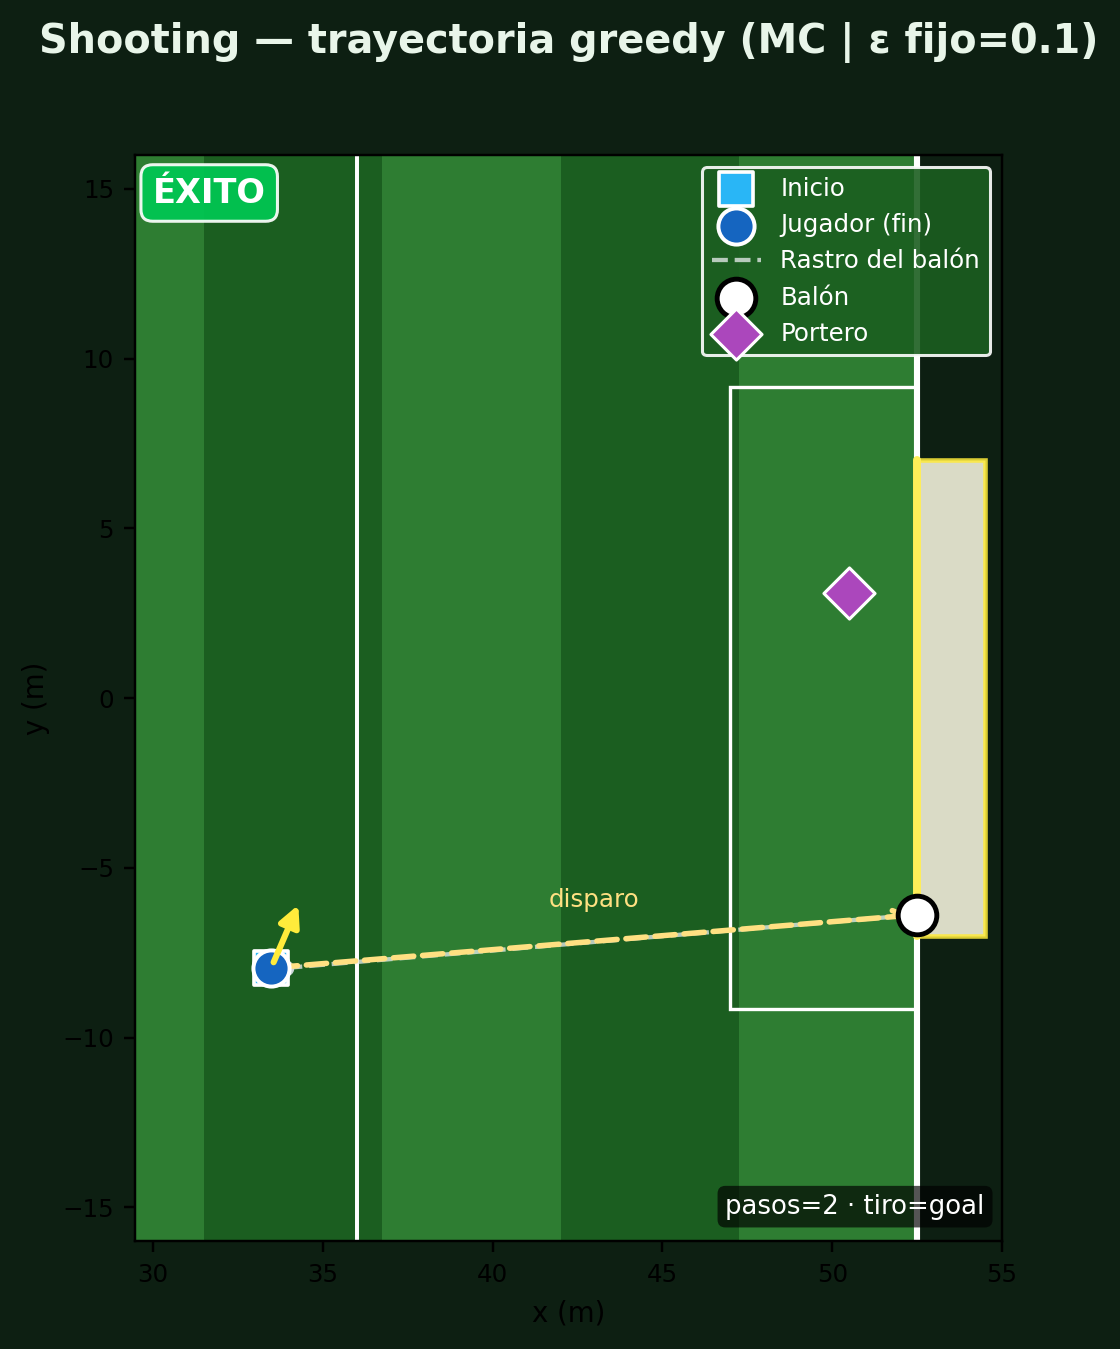
\includegraphics[width=\linewidth]{fig_shooting_tray.png}
        \caption*{Arco abierto}
    \end{subfigure}\hfill
    \begin{subfigure}[t]{0.48\textwidth}
        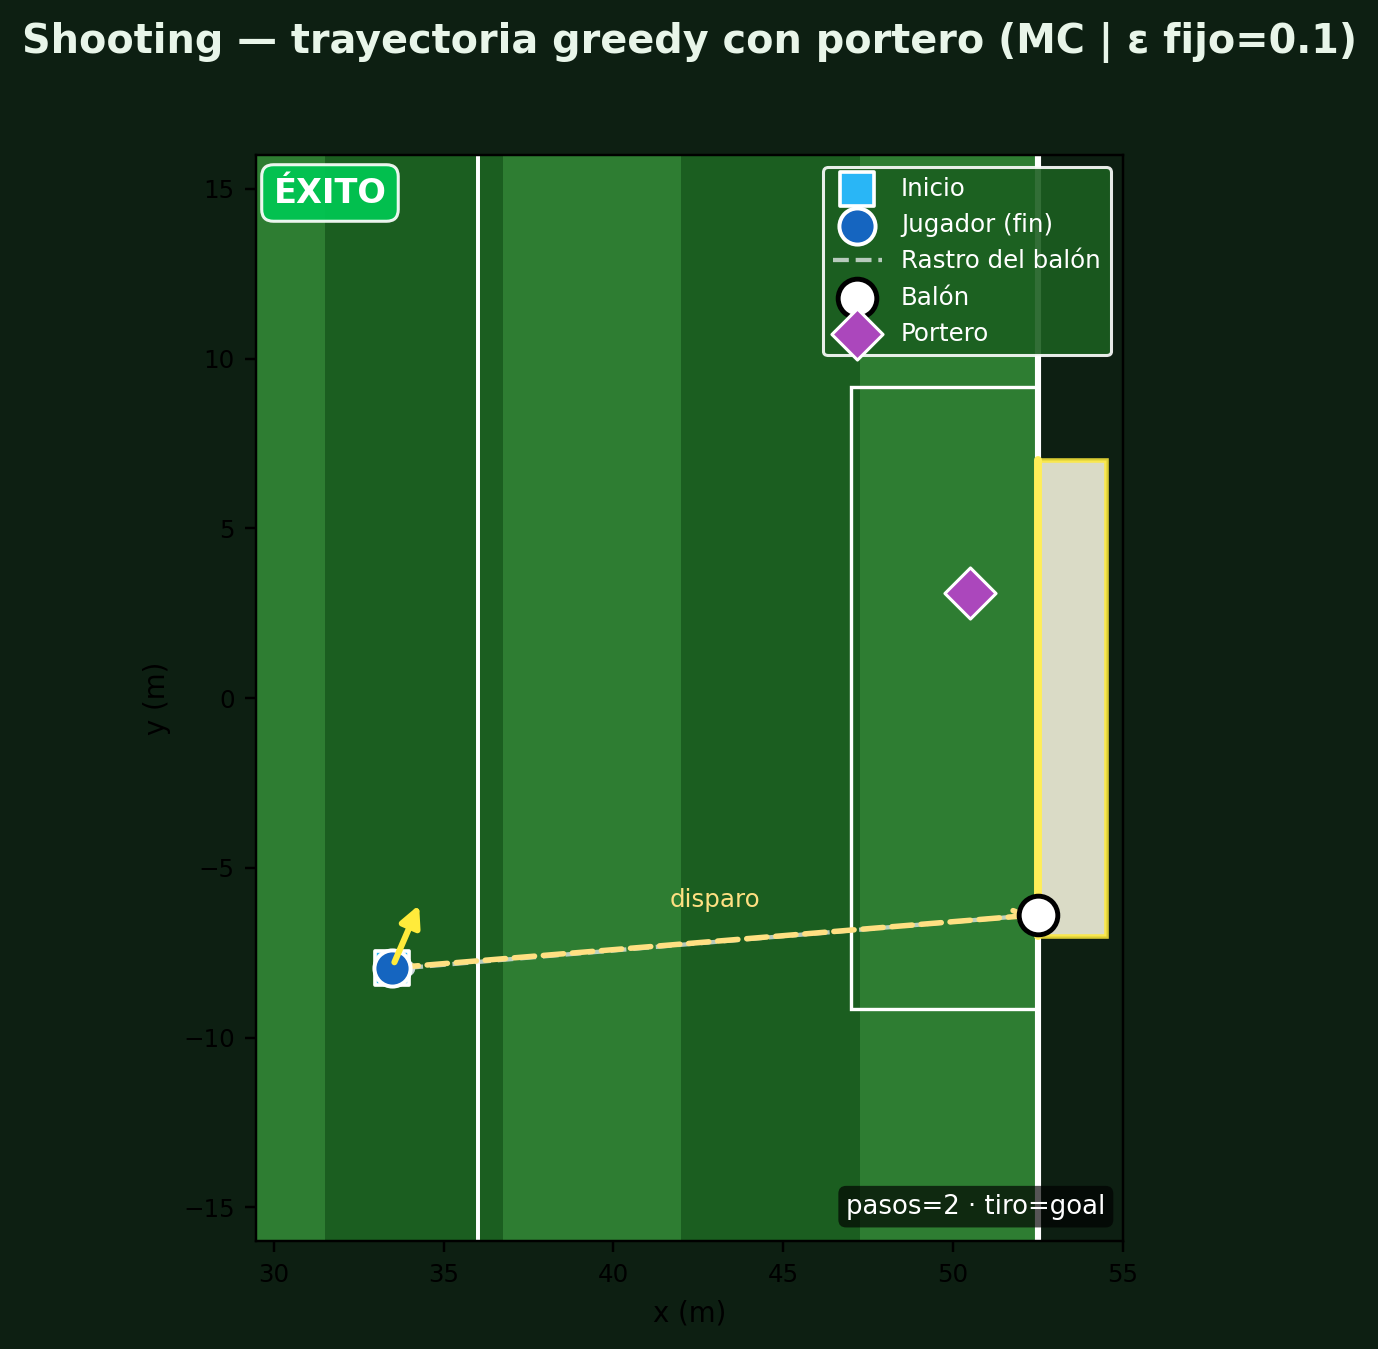
\includegraphics[width=\linewidth]{fig_shooting_tray_gk.png}
        \caption*{Con portero}
    \end{subfigure}
    \caption{Tiro---trayectorias greedy canónicas (open / GK).}
    \label{fig:shot-viz}
\end{figure}

\FloatBarrier
\section{Pase 2v1}
Premiar cada pase con $+30$ inflaba $G_0$ pero no la posesión.
Tras rebalancear (posesión densa, pases moderados, \texttt{ALEJARSE}), el criterio estricto es aprendible.
Con defensor estocástico y stun$=0$ (config adoptada), MC + $\varepsilon$ fijo alcanza $\approx 93\%$ de éxito estricto.

\begin{figure}[htbp]
    \centering
    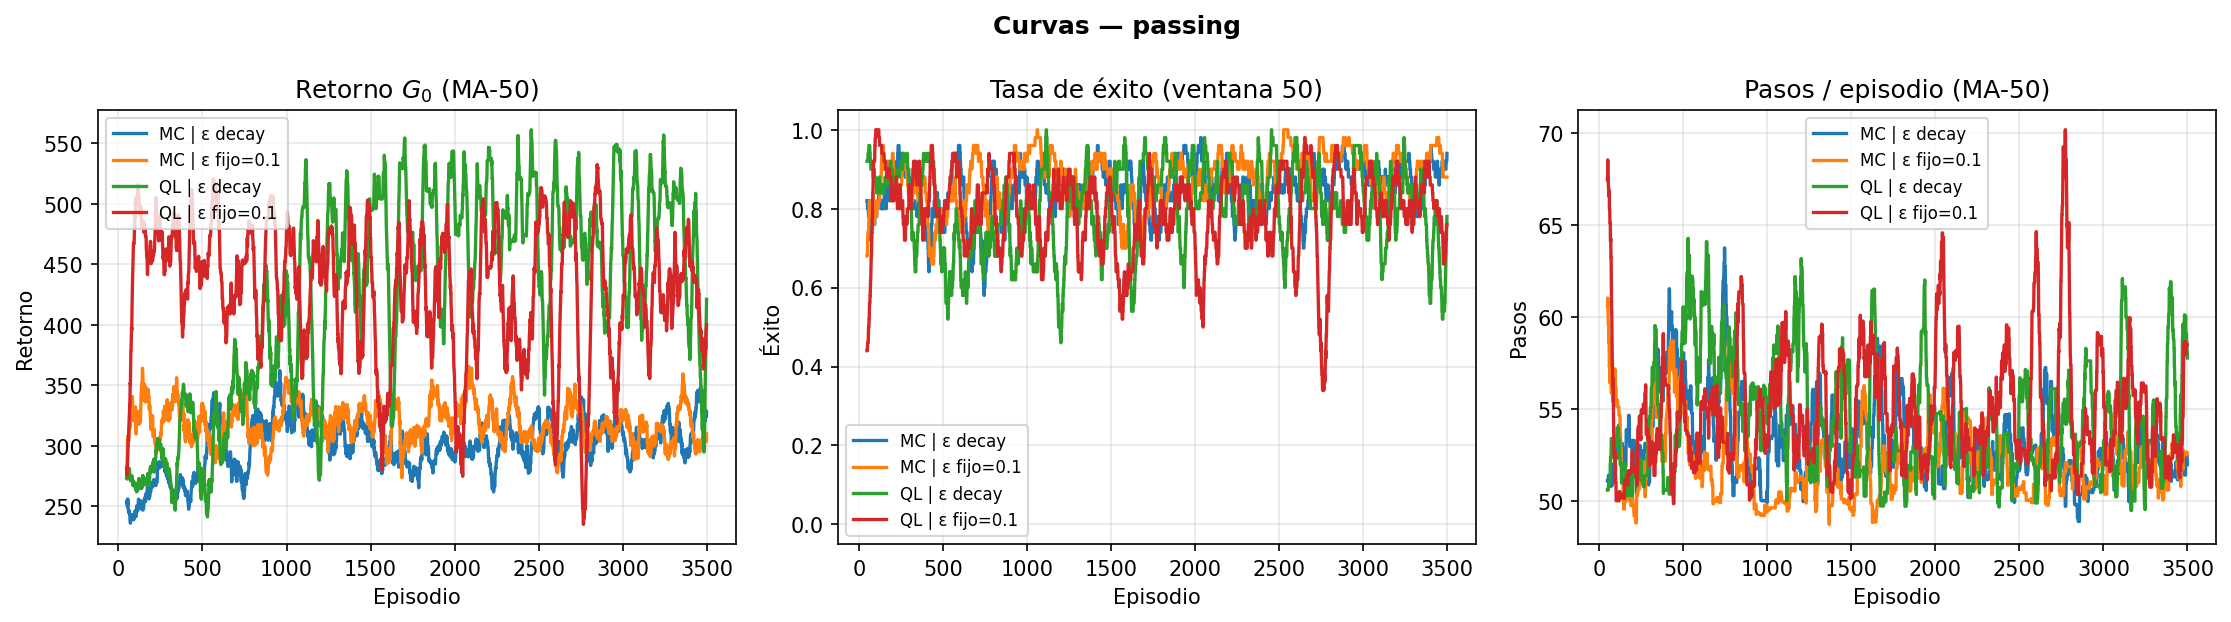
\includegraphics[width=\textwidth]{fig_passing_curvas.png}
    \caption{Pase~2v1---curvas de aprendizaje (stun$=0$). QL infla $G_0$ con muchos pases; el éxito estricto favorece a MC.}
    \label{fig:pass-curvas}
\end{figure}

El \emph{stun} post-pase \textbf{no} está en el enunciado: era un colchón nuestro.
Una ablación (3000 eps, MC/QL, $\varepsilon$ fijo) muestra que se puede \textbf{quitar} sin romper el aprendizaje; subir mucho la velocidad del defensor sí lo degrada.

\begin{table}[htbp]
\centering
\small
\begin{tabular}{@{}lcc@{}}
\toprule
Config.\ defensor & MC éxito & QL éxito \\
\midrule
stun$=3$ (histórico) & $97\%$ & $85\%$ \\
stun$=1$ & $97\%$ & $90\%$ \\
stun$=0$ (adoptado) & $93\%$ & $81\%$ \\
stun$=0$, velocidad $+25\%$ & $77\%$ & $65\%$ \\
stun$=0$, velocidad $+50\%$ & $76\%$ & $72\%$ \\
\bottomrule
\end{tabular}
\caption{Ablación de libertad del defensor (últimos 100 eps; seed~42). Adoptamos stun$=0$ con velocidad base $0.18{+}0.10U$.}
\end{table}

\begin{figure}[htbp]
    \centering
    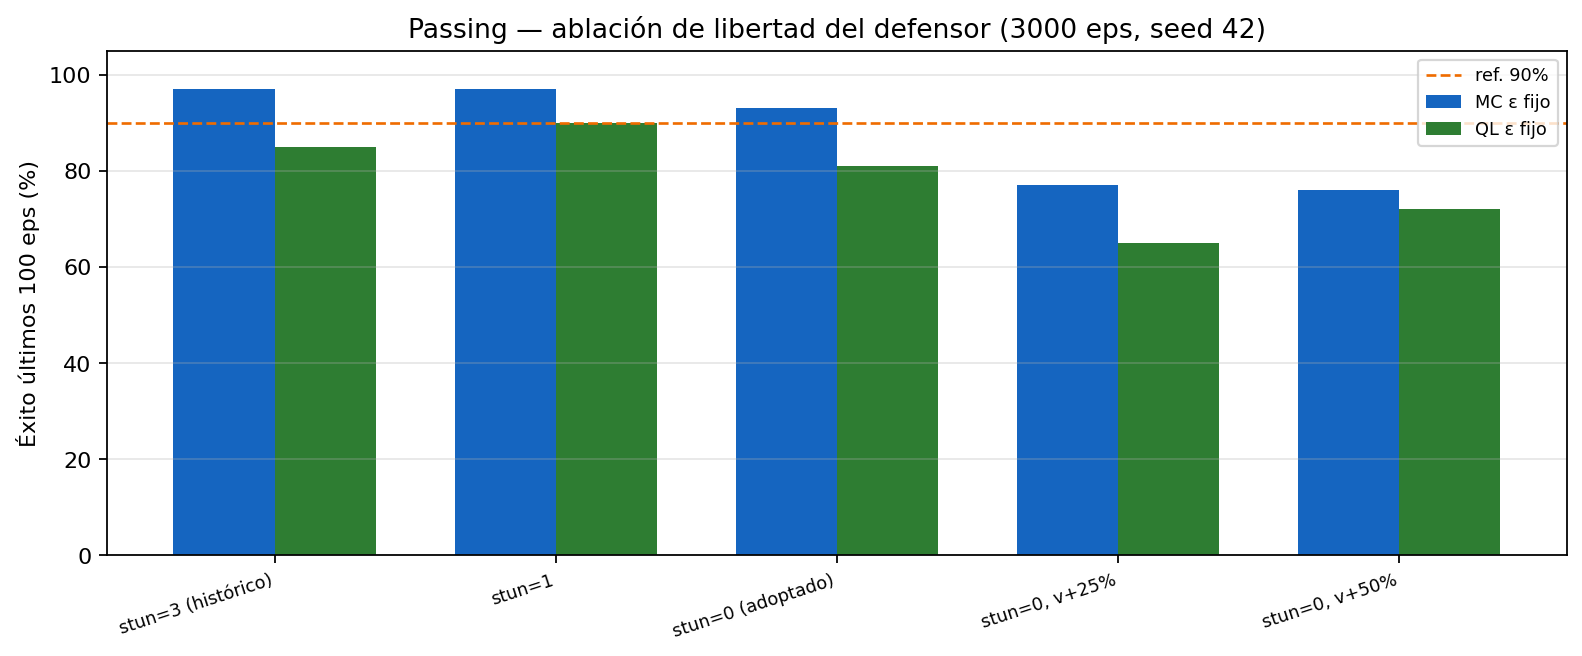
\includegraphics[width=0.88\textwidth]{fig_passing_ablation.png}
    \caption{Passing---éxito vs libertad del defensor (MC/QL, 3000 eps).}
    \label{fig:pass-ablation}
\end{figure}

Con stun$=0$ el rastro del defensor es mucho más largo; con stun$=3$ a menudo apenas se mueve (misma seed abajo).

\begin{figure}[htbp]
    \centering
    \begin{subfigure}[t]{0.48\textwidth}
        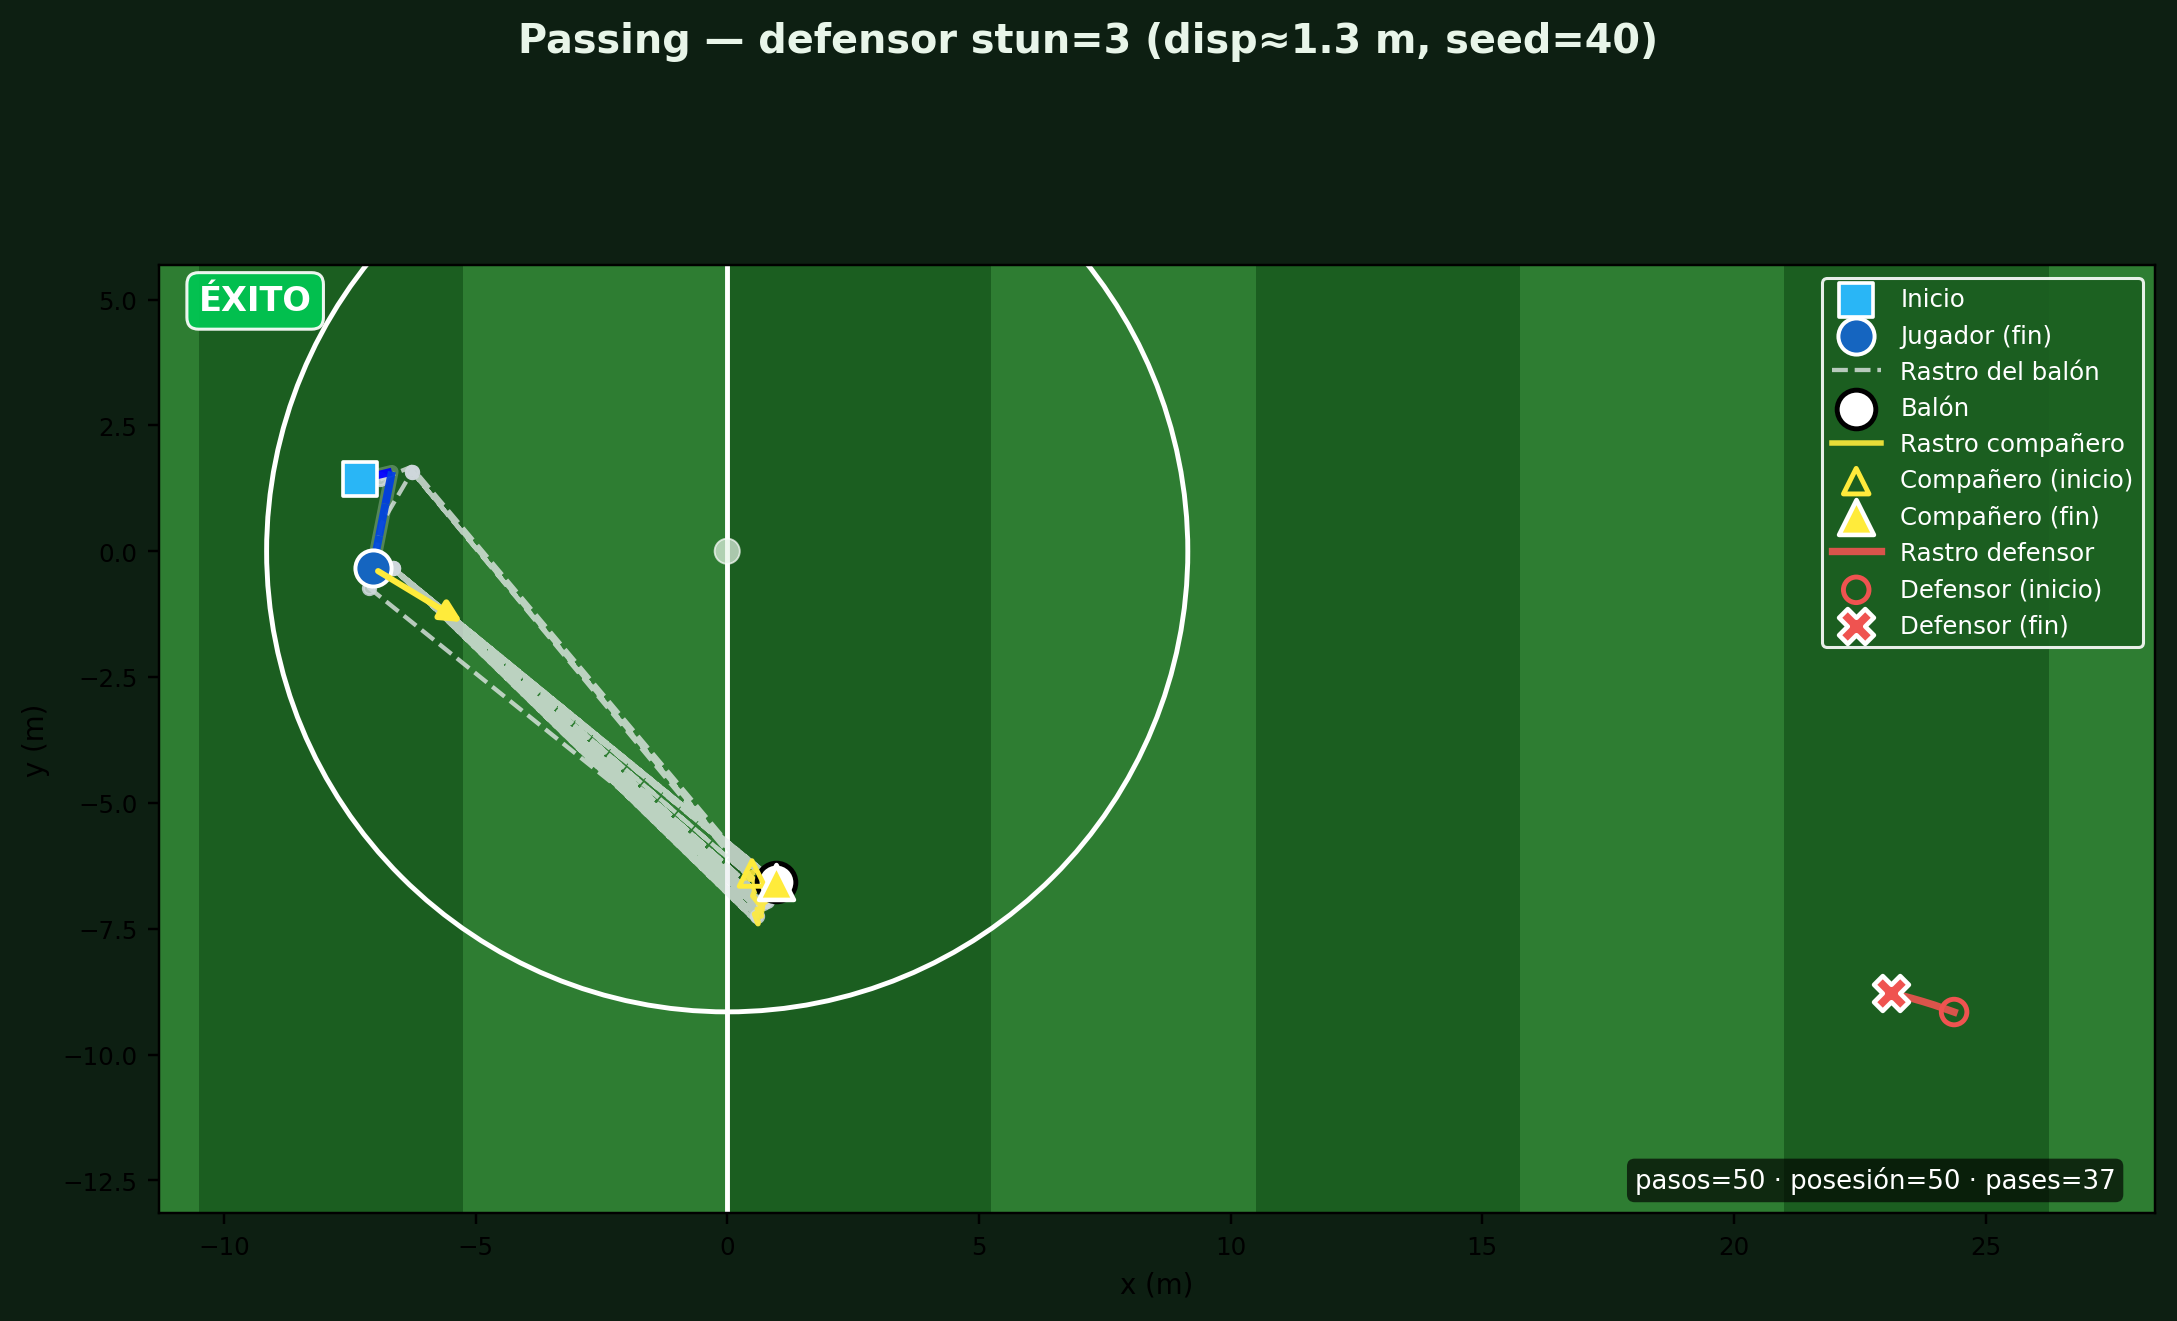
\includegraphics[width=\linewidth]{fig_passing_ablation_stun3.png}
        \caption*{stun$=3$ (disp.\ corta)}
    \end{subfigure}\hfill
    \begin{subfigure}[t]{0.48\textwidth}
        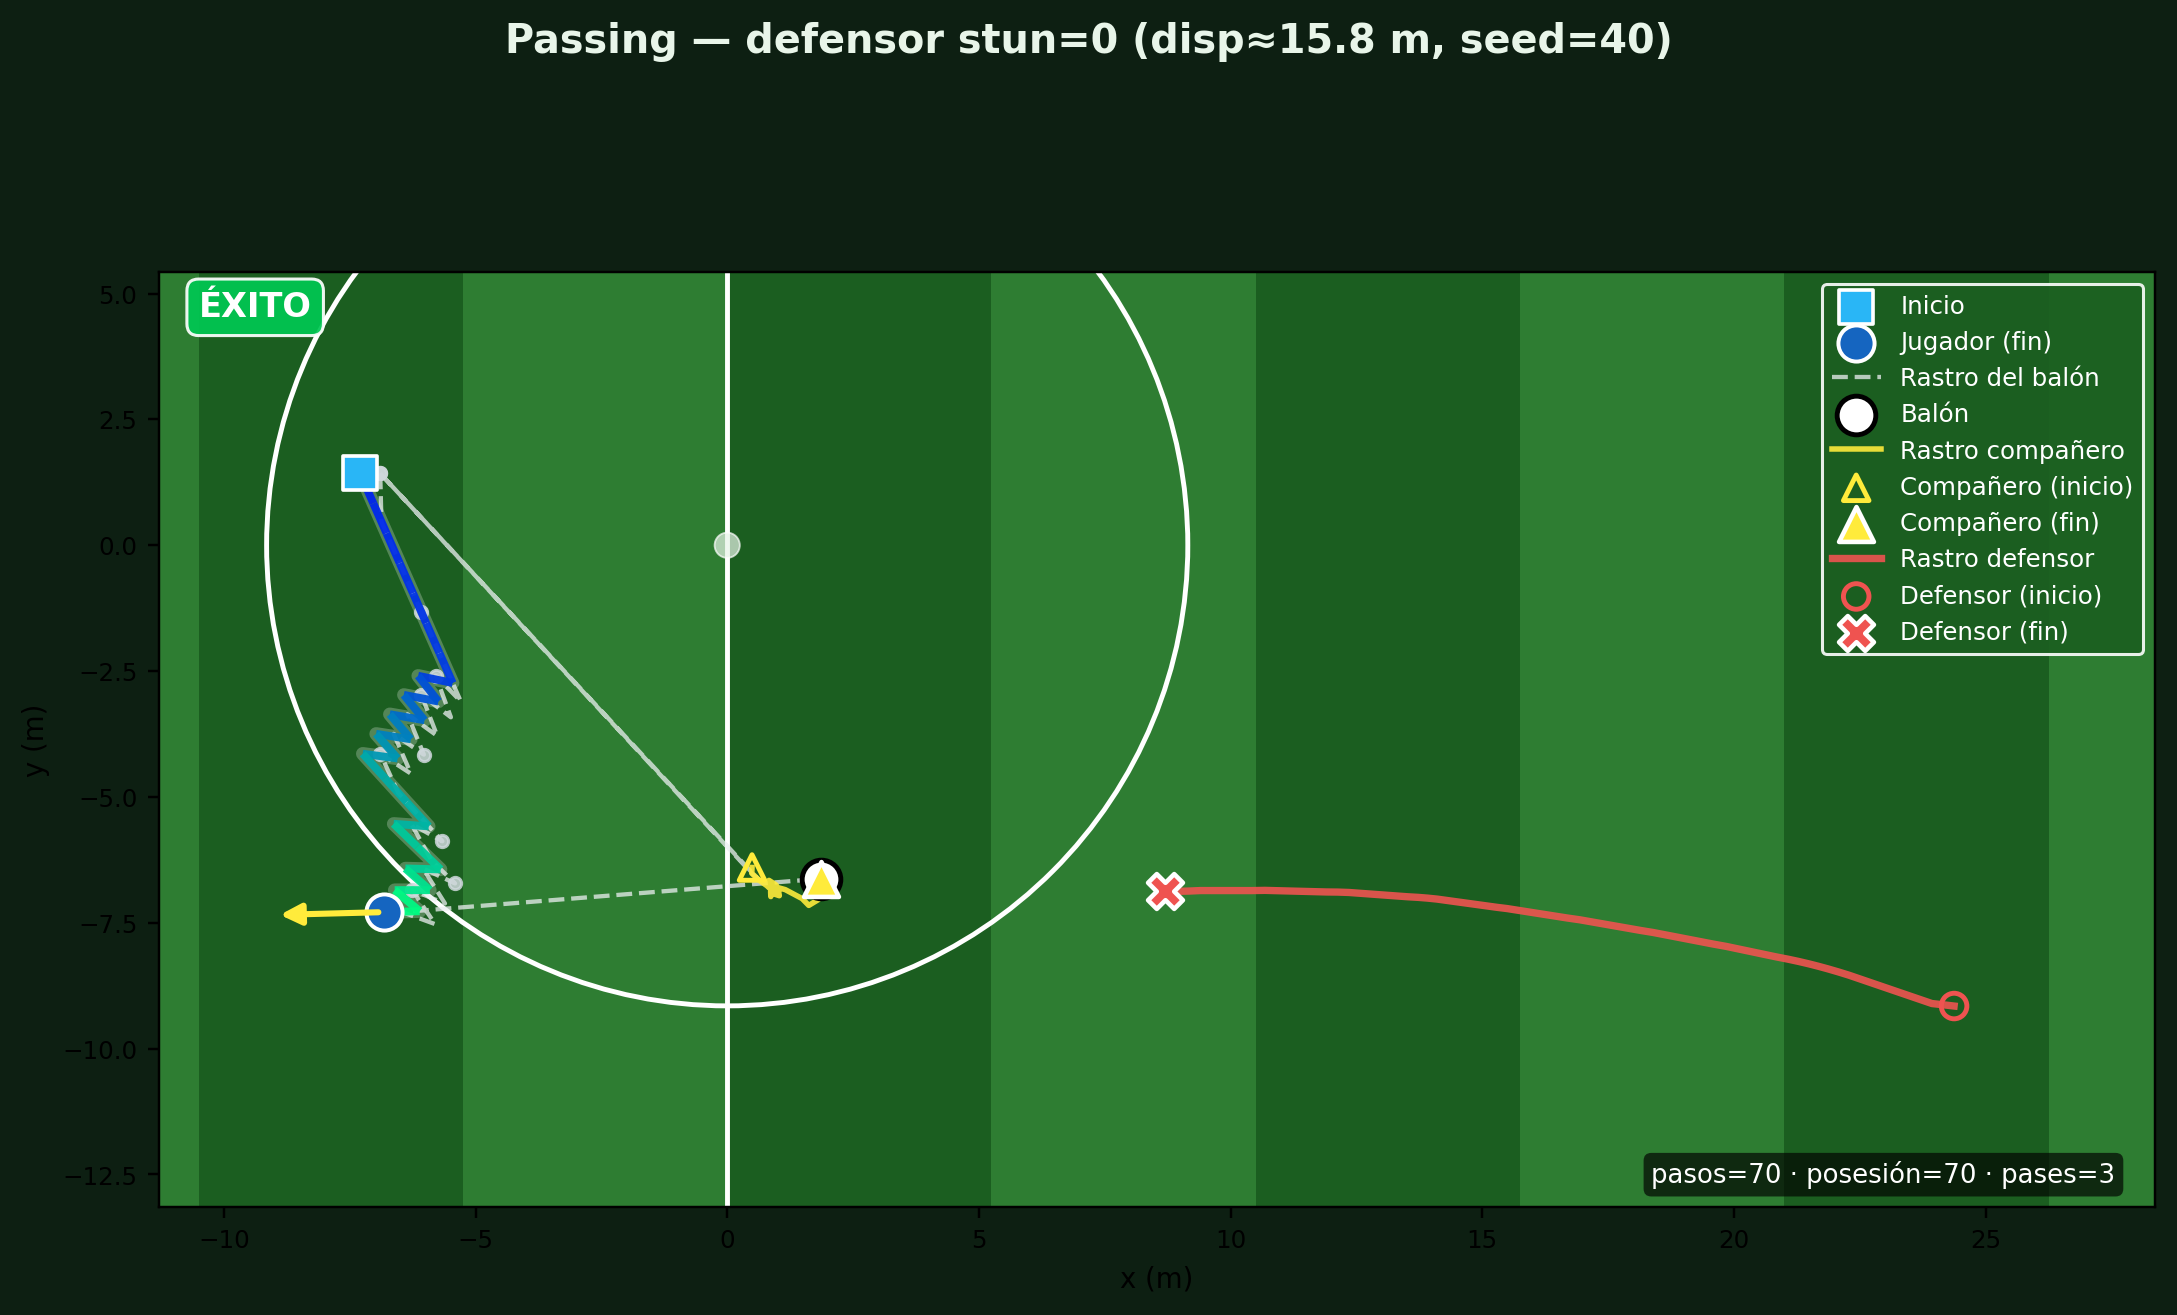
\includegraphics[width=\linewidth]{fig_passing_ablation_stun0.png}
        \caption*{stun$=0$ (disp.\ larga)}
    \end{subfigure}
    \vspace{0.3em}
    \begin{subfigure}[t]{0.48\textwidth}
        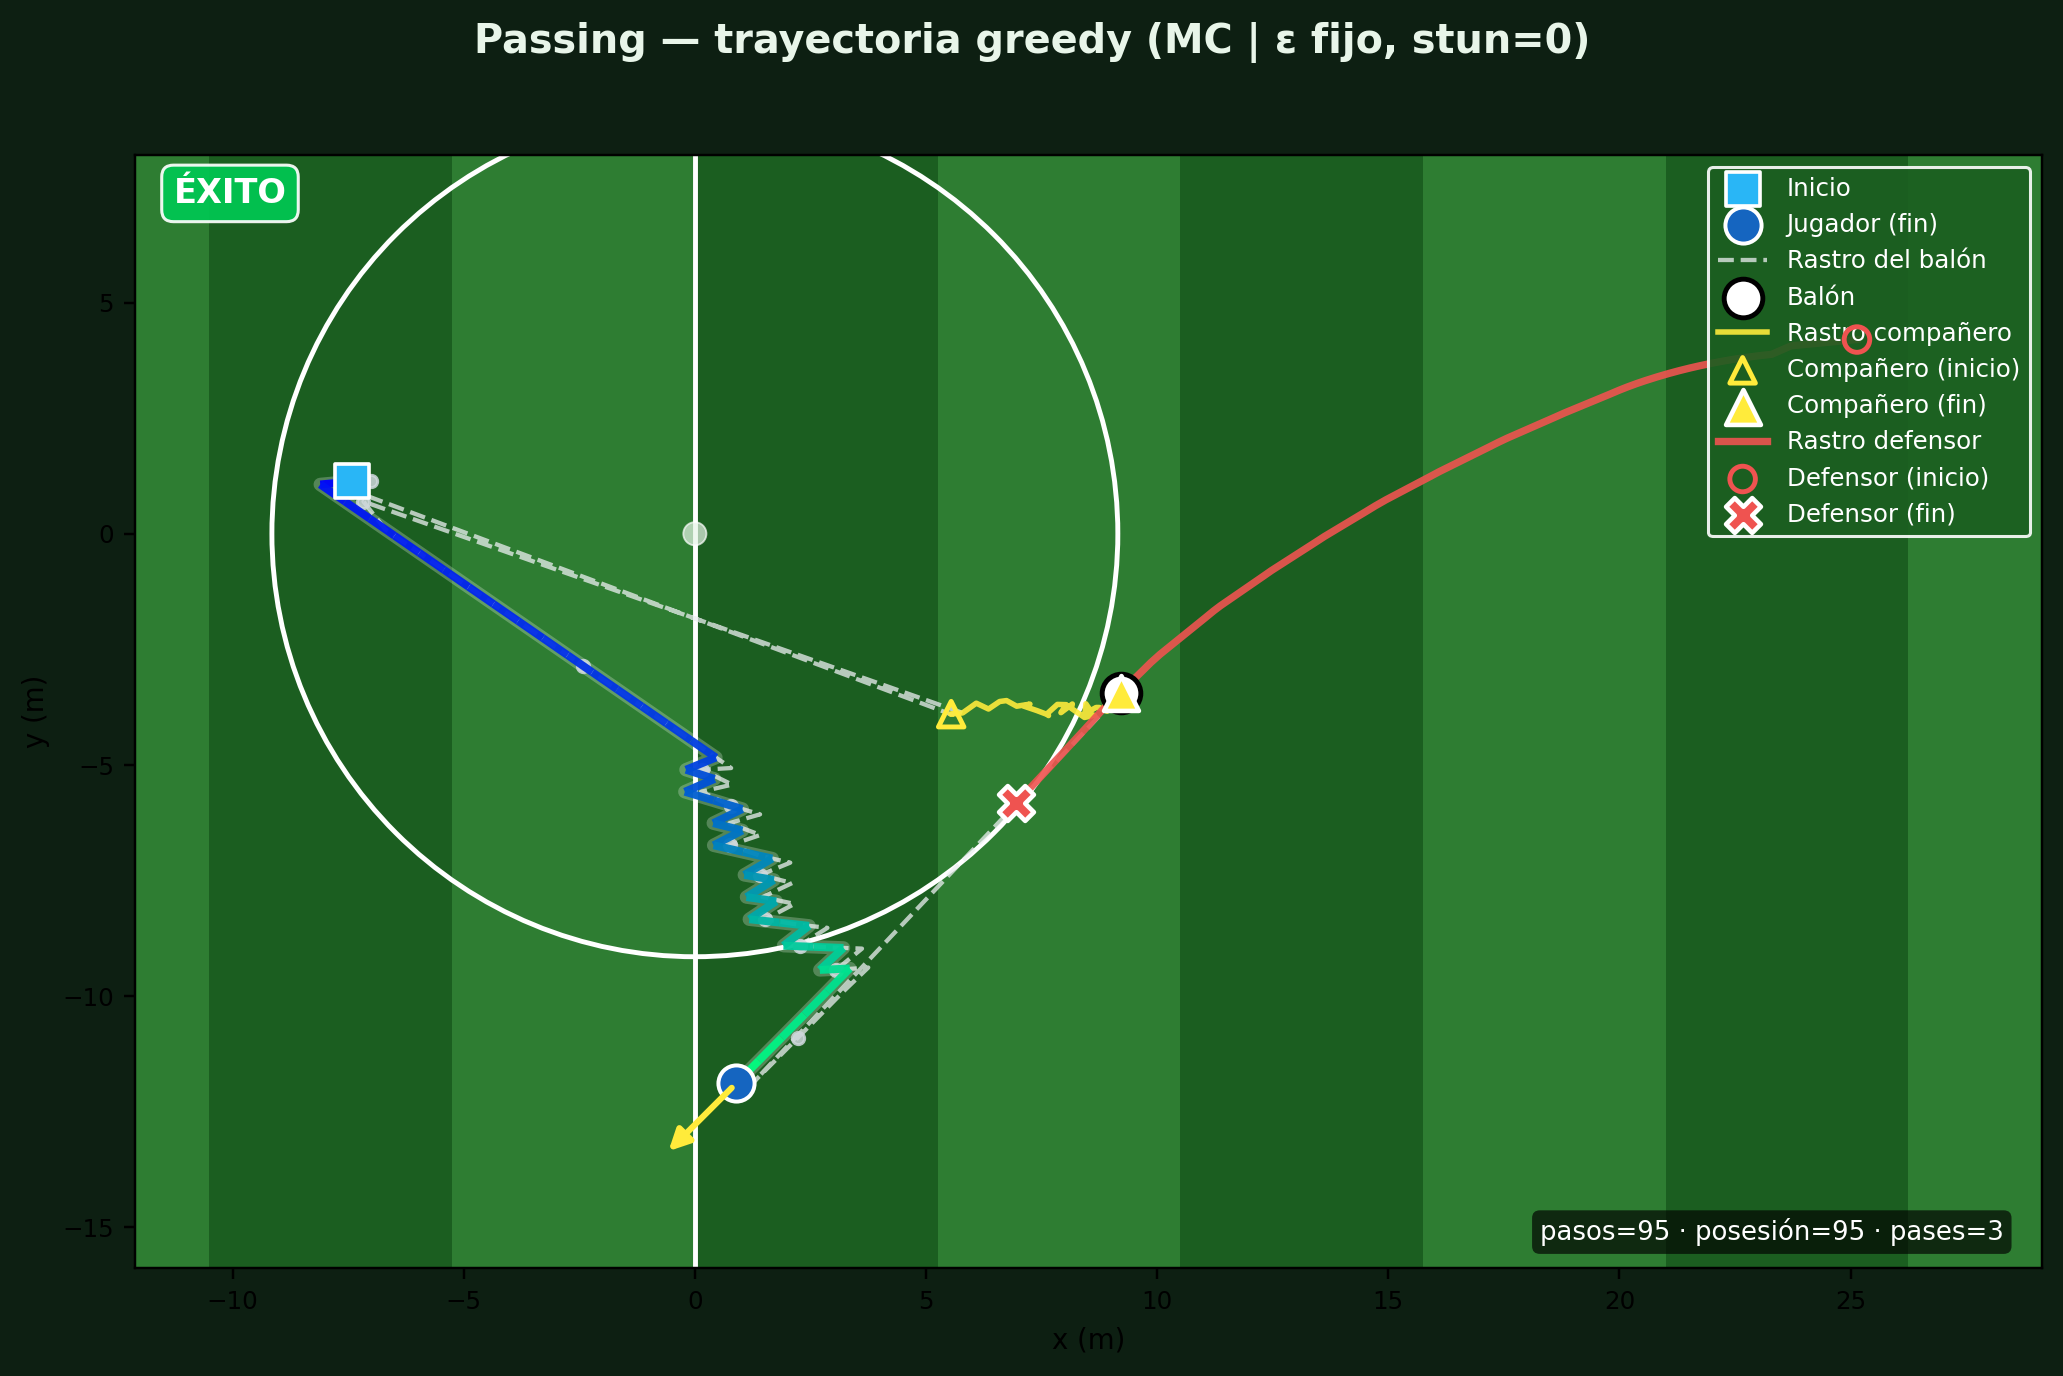
\includegraphics[width=\linewidth]{fig_passing_tray.png}
        \caption*{Canónica adoptada (stun$=0$)}
    \end{subfigure}\hfill
    \begin{subfigure}[t]{0.48\textwidth}
        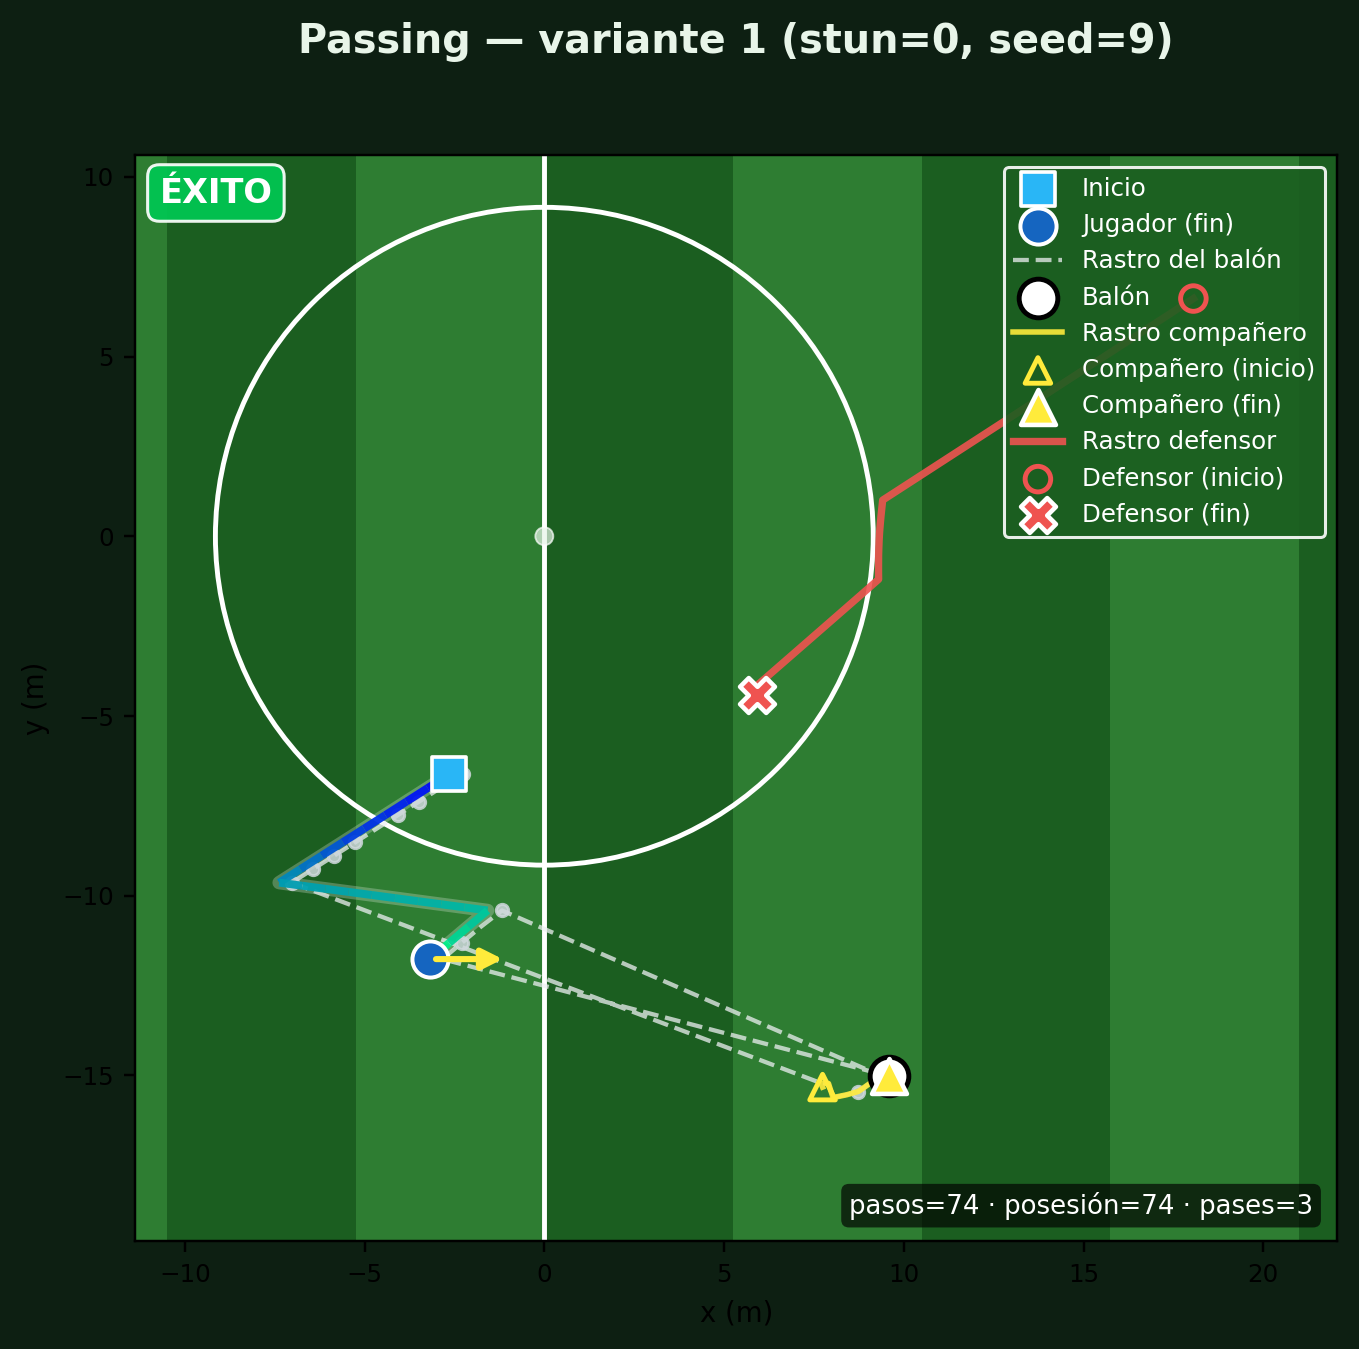
\includegraphics[width=\linewidth]{set_passing_01.png}
        \caption*{Variante stun$=0$}
    \end{subfigure}
    \caption{Pase---ablación visual del stun y trays con defensor libre (rastro rojo).}
    \label{fig:pass-viz}
\end{figure}

\FloatBarrier
\section{Conclusiones}
Cumplimos la Fase~1: cuatro MDPs con discretización justificada, MC Control y Q-Learning, $\varepsilon$ fijo vs decay, curvas, $V^*$/$\pi^*$, trayectorias y umbrales del enunciado.

\begin{itemize}
    \item \textbf{Discretizar con criterio.} Bins polares anclados al kickable ($0.8$\,m) y a conos de dash/giro; cada tarea extiende esa base (meta, GK, compañero/defensor).
    \item \textbf{Pipeline uniforme.} El mismo código de agentes/métricas sirve a las cuatro tareas si el contrato del env es homogéneo.
    \item \textbf{Exploración importa.} En persecución, MC con $\varepsilon$ fijo no limpia timeouts en distancias largas; con decay sí. En tiro y pase, $\varepsilon$ fijo ayuda a seguir muestreando acciones útiles.
    \item \textbf{No hay ganador único.} Persecución/drible (caminos largos, shaping denso) $\rightarrow$ \textbf{QL + $\varepsilon$ decay}.
    Tiro (ruido, pocas decisiones) y pase ($R$ $\neq$ criterio del enunciado) $\rightarrow$ \textbf{MC + $\varepsilon$ fijo}: el retorno episódico y la exploración constante estiman mejor kicks/macros; QL infla $G_0$ localmente (p.\ ej.\ spamear pases) con peor éxito estricto.
    El cuello de botella es la profundidad temporal o la alineación $R\leftrightarrow$ criterio.
    \item \textbf{Shaping amarrado al enunciado.} En pase, premiar pases sin posesión densa falló; rediseñamos $R$ y, en ablación, quitamos el stun post-pase (colchón nuestro, no requisito del curso).
    \item \textbf{Límite del proxy.} Sin visión ruidosa ni estamina; revalidar en \texttt{rcssserver}. Fase~2: DQN/PPO y jerarquías sobre estas skills.
\end{itemize}

\begin{thebibliography}{9}
\bibitem{sutton}
R. S. Sutton and A. G. Barto, \textit{Reinforcement Learning: An Introduction}, 2nd ed., MIT Press, 2018.
\bibitem{robocup}
H. Kitano et al., ``The RoboCup Soccer Server,'' in \textit{RoboCup-97}, Springer, 1998.
\bibitem{ng1999}
A. Y. Ng, D. Harada, and S. Russell, ``Policy invariance under reward transformations,'' in \textit{ICML}, 1999.
\end{thebibliography}

\end{document}
